\chapter{电网络}
\label{chap:graph-electrical-networks}

在四点环加对角边$13$的图上，从顶点$1$送入一单位电流，从顶点$3$取出。电流可以直接走对角边，也可以沿环上的两条外侧支路绕行。怎样在这些支路之间分配电流，取决于各条边的电阻。分配确定后，维持单位电流所需要的两端电势差，就概括了整张网络对这一对顶点的作用。

我们先分别写出逐边的电势与电流关系，以及逐点的流入流出平衡。把两个条件联立后，未知量只剩各顶点的电势，系数矩阵正是第~\ref{chap:graph-laplacian-matrix}章的组合拉普拉斯。解出电势，就能沿边恢复电流。

还可以把不同的分流方案放在一起比较耗散。在给定注入下，实际电流是所有守恒分流中耗散最小的，这就是Thomson原理。从单位分流所需的端点压降，可以引出有效电阻。它在后面的稀疏化抽样与往返时间计算中都有直接用途。

\section{电网络的基本定律}
\label{sec:electrical-network-laws}

把带正权边的无向图看成\term{电网络}（electrical network）：每条正权边是一个电阻元件，顶点是这些元件连接的接点，外部可以在指定接点注入或取出电流。我们先从一个接点看各条边的净流量，建立电流守恒方程；再从一条边看两端电势怎样决定流过它的电流，写出Ohm定律。

\subsection{电流守恒}
\label{sec:electrical-current-conservation}

一条边导电的容易程度用\term{电导}（conductance）$c_e = w_e > 0$来衡量，倒数$r_e = 1/c_e$是\term{电阻}（resistance）。电导越大，同样的电势差下流过的电流越多。零权边不导电，删去它们后保留的图称为正权支撑。正权支撑仍包括所有顶点，即使某个顶点不再与任何正权边相邻。

设顶点数为$n$，正权边数为$m$。每条边记录一个带符号的电流，组成向量$\bm f\in\mathbb R^m$。记录方向沿用第~\ref{chap:graph-incidence-matrix}章的约定：关联矩阵$\bm B\in\mathbb R^{n\times m}$的每列在尾端取$+1$、头端取$-1$。$f_e > 0$表示电流沿记录方向流动，$f_e < 0$表示实际流向与记录相反。

以四点图为例。边$41$的记录方向为$4\to1$。若边上流量为$-2$，实际含义是$2$个单位的电流从$1$流向$4$。看顶点$1$，这条边从外面带来了$2$个单位的电流。

每个顶点的进出必须平衡。由关联矩阵按行读取，顶点$i$在出发边上取$+f_e$，在到达边上取$-f_e$，各项相加得到净流出量$(\bm B\bm f)_i$。假设两条边的记录方向都朝外，其流量分别为$3$和$-1$。实际上前者送出$3$，后者从外面送入$1$，净流出$3 - 1 = 2$。

外部在顶点$i$注入电流$b_i$，这些电流必须从该点流向网络内部。$b_i > 0$是注入，$b_i < 0$是引出。\term{Kirchhoff电流定律}（Kirchhoff's current law）要求每个顶点的网络净流出等于外部注入：
\begin{equation}
  \bm B\bm f = \bm b.
  \label{eq:electrical-current-conservation}
\end{equation}
上面那个接点的净流出为$2$，所以外部恰好需要送入$b_i = 2$单位电流来维持平衡。

图~\ref{fig:electrical-local-current-balance}把同一个接点的电流守恒用两种方式画出来。左图用记录方向和带符号的数值。右图把方向转成实际流向，在接点处画出外部注入的量。

\begin{BookInlineFigure}
  \centering
  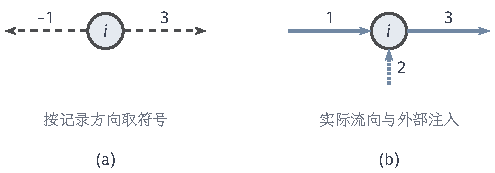
\includegraphics[scale=1]{figures/03-graphs/05-matrices-and-spectra/tikz/electrical-local-current-balance/figure.pdf}
  \caption{接点的电流守恒。(a)~虚线箭头给出两条边的记录方向，左边的负号表示逆向流动。(b)~两条实线箭头给出真实流向，下方点线箭头给出维持守恒所需的外部注入量。}
  \label{fig:electrical-local-current-balance}
\end{BookInlineFigure}

把式~\eqref{eq:electrical-current-conservation}的$n$个方程按顶点求和。每条边在尾端贡献$+f_e$，在头端贡献$-f_e$，两者抵消。因此全图的外部注入总和必须为零：
\[
  \sum_{i=1}^n b_i = \bm 1^\top \bm b = 0.
\]
对单个连通分量也一样——如果两个分量之间没有正电导边，电流就无法从一个分量穿越到另一个。每个正权连通分量必须各自满足注入总量为零。

\subsection{Ohm定律}
\label{sec:electrical-ohm-law}

守恒只限制流入和流出的总量，还没有决定每条边上有多少电流。每条边的电流由两端的电势差和该边的电导共同决定。

给每个顶点一个电势值$v_i$，组成向量$\bm v\in\mathbb R^n$。沿边$e\colon i\to j$看，电势从$v_i$变到$v_j$，沿记录方向的压降为$v_i - v_j$。例如$v_i = 3$、$v_j = 1$，压降为$2$。若这条边的电导为$c_e = 1/2$，\term{Ohm定律}（Ohm's law）给出流过它的电流：
\[
  f_e = c_e(v_i - v_j) = \tfrac{1}{2} \times 2 = 1.
\]
压降越大或电导越大，电流越大。

对所有记录边一起取差，得到压降向量$\bm B^\top\bm v$。再在每条边上乘以该边的电导，便得到全部电流：
\begin{equation}
  \bm f = \bm C\bm B^\top\bm v, \qquad \bm C = \operatorname{diag}(c_e\colon e\in E).
  \label{eq:electrical-ohm-law}
\end{equation}

沿任一闭环累计压降，中间顶点的电势在前一步的末端和后一步的始端各出现一次，正好抵消。在四点图上，沿$1\to2\to3\to1$走一圈：
\[
  (v_1 - v_2) + (v_2 - v_3) + (v_3 - v_1) = 0.
\]
这就是\term{Kirchhoff电压定律}（Kirchhoff's voltage law）。它说明由顶点电势产生的压降向量一定落在第~\ref{chap:graph-incidence-matrix}章的割空间$\operatorname{im}\bm B^\top$中。沿环检验时，若已知边电流$f_e$，先乘电阻得到压降$r_e f_e$，再按行进方向加减。

把所有电势同时加上同一个常数$c$，各条边的压降为$(v_i + c) - (v_j + c) = v_i - v_j$，保持不变。因此电流也不会改变。这个常数自由度说明，单靠注入量无法唯一确定电势本身，但可以确定电势差和边电流。下一节求解时，我们会选一个顶点固定电势基准来消去这个自由度。

\section{拉普拉斯方程的求解}
\label{sec:graph-laplacian-solve}

给定各顶点的外部注入电流$\bm b\in\mathbb R^n$，将上一节的Ohm定律与Kirchhoff电流定律联立，即可导出仅含顶点电势$\bm v\in\mathbb R^n$的线性方程组。具体分三步完成：

第一步，用顶点电势表示边压降。由关联矩阵转置的作用，全图$m$条有向参考边上的压降向量为$\Delta\bm v = \bm B^\top\bm v$，其中第$e\colon i\to j$条边的分量为$v_i - v_j$。

第二步，由Ohm定律写出边电流。将每条边的压降乘以该边电导$c_e$，得到边电流向量式~\eqref{eq:electrical-ohm-law}：
\[
  \bm f = \bm C\bm B^\top\bm v.
\]

第三步，代入Kirchhoff电流定律。将$\bm f = \bm C\bm B^\top\bm v$代入守恒方程$\bm B\bm f = \bm b$，消去中间变量$\bm f$，得到
\[
  \bm B\bm C\bm B^\top\bm v = \bm b.
\]
对比第~\ref{sec:graph-laplacian}节的关联矩阵分解式~\eqref{eq:graph-laplacian-incidence-factorization}，左侧的复合矩阵$\bm B\bm C\bm B^\top$正是图的组合拉普拉斯矩阵$\bm L=\bm D-\bm W$（其中边权取为电导$w_{i,j}=c_{i,j}$）。于是电网络的平衡条件归结为如下\emph{拉普拉斯方程}：
\begin{equation}
  \bm L\bm v = \bm b, \qquad \bm L = \bm B\bm C\bm B^\top = \bm D - \bm W.
  \label{eq:electrical-laplacian-system}
\end{equation}
按第$i$个顶点展开，式~\eqref{eq:electrical-laplacian-system}的第$i$行方程为
\[
  (\bm L\bm v)_i = \sum_{j=1}^n c_{i,j}(v_i - v_j) = d_i v_i - \sum_{j=1}^n c_{i,j}v_j = b_i,
\]
其物理含义十分直观：从顶点$i$经所有相邻电阻支路流向邻居的电流之和$\sum_j c_{i,j}(v_i-v_j)$，必须等于外部在顶点$i$注入的电流$b_i$。

本节先证明拉普拉斯方程$\bm L\bm v=\bm b$的可解性充要条件与解空间结构，再说明如何通过选定一个接地点消去电势的常数平移自由度以获得唯一解，随后介绍一般网络的数值求解方法，最后给出树网络上的线性时间求解算法。

\subsection{拉普拉斯方程的可解性}
\label{sec:electrical-laplacian-derivation}

因为组合拉普拉斯矩阵$\bm L$满足$\bm L\bm 1=\bm 0$，它是奇异矩阵（不可逆），并非对任意右端向量$\bm b$都有解。下面的定理给出了拉普拉斯方程$\bm L\bm v=\bm b$有解的充要条件以及全部解的结构。

\begin{theorem}[拉普拉斯方程的可解性与解集结构]
\label{thm:electrical-laplacian-solvability}
设有限无向电网络的正权支撑连通，组合拉普拉斯矩阵为$\bm L\in\mathbb R^{n\times n}$。
\begin{enumerate}
  \item 线性方程组$\bm L\bm v=\bm b$有解，当且仅当全图外部注入电流的总和为零：
  \begin{equation}
    \bm 1^\top\bm b = \sum_{i=1}^n b_i = 0.
    \label{eq:electrical-zero-sum-condition}
  \end{equation}
  \item 当$\bm 1^\top\bm b=0$时，若$\bm v_0$是一个特解，则方程组$\bm L\bm v=\bm b$的通解为
  \[
    \bm v = \bm v_0 + c\bm 1 \qquad (c\in\mathbb R),
  \]
  即任意两组电势解仅相差一个全局常数平移$c\bm 1$；所有电势解经Ohm定律生成的边电流向量$\bm f=\bm C\bm B^\top\bm v$唯一确定。
  \item 在满足$\bm 1^\top\bm v=0$的零均值子空间$\bm 1^\perp$内，方程组$\bm L\bm v=\bm b$存在唯一解，由Moore--Penrose伪逆给出：$\bm v_{\mathrm{zm}} = \bm L^\dagger\bm b$。
\end{enumerate}
\end{theorem}

\begin{proof}
（1）由定理~\ref{thm:graph-laplacian-components}，当正权支撑连通时，$\bm L$的零空间为一维常向量空间$\ker\bm L=\operatorname{span}\{\bm 1\}$。由于$\bm L$是实对称矩阵，其列空间（像空间）等于零空间的正交补：
\[
  \operatorname{im}\bm L = (\ker\bm L)^\perp = \bm 1^\perp = \Bigl\{\bm b\in\mathbb R^n : \bm 1^\top\bm b = 0\Bigr\}.
\]
因此$\bm b\in\operatorname{im}\bm L$（即$\bm L\bm v=\bm b$有解）当且仅当$\bm 1^\top\bm b = 0$。

（2）设$\bm v_1,\bm v_2$均满足$\bm L\bm v=\bm b$，作差得$\bm L(\bm v_1-\bm v_2)=\bm 0$，即$\bm v_1-\bm v_2\in\ker\bm L=\operatorname{span}\{\bm 1\}$，故存在常数$c\in\mathbb R$使得$\bm v_2=\bm v_1+c\bm 1$。代入Ohm定律，因$\bm B^\top\bm 1=\bm 0$，有
\[
  \bm C\bm B^\top\bm v_2 = \bm C\bm B^\top(\bm v_1 + c\bm 1) = \bm C\bm B^\top\bm v_1,
\]
故边电流向量唯一确定。

（3）由于$\ker\bm L=\operatorname{span}\{\bm 1\}$且$\operatorname{im}\bm L=\bm 1^\perp$，$\bm L$限制在不变子空间$\bm 1^\perp$上是到自身的对称正定可逆算子（$n\geq2$时最小特征值为$\lambda_2>0$；单点网络的零和空间只有零向量），其逆算子在$\bm 1^\perp$上正是Moore--Penrose伪逆$\bm L^\dagger$，故唯一零均值解为$\bm v_{\mathrm{zm}}=\bm L^\dagger\bm b$。
\end{proof}

若正权支撑不连通，有$c$个连通分量$V_1,\ldots,V_c$，则由$\ker\bm L=\operatorname{span}\{\bm 1_{V_1},\ldots,\bm 1_{V_c}\}$可知：$\bm L\bm v=\bm b$有解当且仅当每个连通分量内部的外部注入总和各自为零（$\bm 1_{V_a}^\top\bm b=0$，$a=1,\ldots,c$），此时各连通分量的电势可独立平移各自的常数。

\subsection{接地与唯一解}
\label{sec:electrical-grounding}

定理~\ref{thm:electrical-laplacian-solvability}表明，在连通网络中，同一组相容注入$\bm b$对应无穷多组相差常数平移的电势解。为了在实际计算中直接通过可逆方阵唯一解出各点电势，最简便的做法是选定某个参考顶点$q\in V$，将其电势固定为零：
\[
  v_q = 0.
\]
这一操作称为在顶点$q$处\term{接地}（grounding）。例如三点电势$(5,3,2)^\top$在第三个顶点接地后，整体减去基准值$2$，即唯一确定为$(3,1,0)^\top$。

在选定接地点$q$并令$v_q=0$后，第$q$列在矩阵乘积$\bm L\bm v$中的贡献恒为$v_q\bm L_{:,q}=\bm 0$，因此可以直接删去$\bm L$的第$q$列；同时，由于全部$n$个顶点的守恒方程之和恒为零，只要其余$n-1$个顶点的守恒方程得到满足，第$q$个顶点的守恒方程就会自动满足，因此也可以删去$\bm L$的第$q$行。记从$\bm L$中删去第$q$行和第$q$列所得的$(n-1)\times(n-1)$主子矩阵为$\overline{\bm L}$，同时从$\bm v$和$\bm b$中删去第$q$个分量得到$\overline{\bm v},\overline{\bm b}\in\mathbb R^{n-1}$。

需要特别注意，删去第$q$行和第$q$列并不意味着把接地点$q$关联的边从电路中剪断：若边$e$连接保留顶点$i$与接地点$q$，它在第$i$行方程中原本贡献$c_e(v_i - v_q)$，代入$v_q = 0$后变为$c_e v_i$，该电导$c_e$依然保留在$\overline{\bm L}$的第$i$个对角元$d_i$中。

\begin{theorem}[接地约化系统的正定性与唯一解]
\label{prop:electrical-grounded-system}
设有限无向电网络的正权支撑连通，任选顶点$q\in V$接地（令$v_q=0$）。则删去$\bm L$的第$q$行和第$q$列所得的约化拉普拉斯矩阵$\overline{\bm L}\in\mathbb R^{(n-1)\times(n-1)}$是对称正定矩阵。对任意满足$\bm 1^\top\bm b=0$的注入向量$\bm b\in\mathbb R^n$，约化方程组
\begin{equation}
  \overline{\bm L}\,\overline{\bm v} = \overline{\bm b}
  \label{eq:electrical-grounded-system}
\end{equation}
存在唯一解$\overline{\bm v}=\overline{\bm L}^{-1}\overline{\bm b}$；将其在第$q$个位置补入$v_q=0$后，即得原方程组$\bm L\bm v=\bm b$满足$v_q=0$的唯一电势解。
\end{theorem}

\begin{proof}
第一步，证明$\overline{\bm L}$对称正定。$\overline{\bm L}$作为实对称矩阵$\bm L$的主子矩阵显然对称。任取非零向量$\overline{\bm x}\in\mathbb R^{n-1}$，在第$q$个位置补入$x_q=0$延拓为$n$维向量$\bm x\in\mathbb R^n$。由于$\overline{\bm x}\neq\bm 0$而$x_q=0$，$\bm x$的各个分量不全相等，故$\bm x\notin\operatorname{span}\{\bm 1\}=\ker\bm L$。由定理~\ref{prop:graph-laplacian-quadratic-form}(1)与定理~\ref{thm:graph-laplacian-components}，得
\[
  \overline{\bm x}^\top \overline{\bm L}\,\overline{\bm x}
  = \bm x^\top \bm L \bm x > 0.
\]
因此$\overline{\bm L}$是对称正定矩阵，从而可逆（这也与第~\ref{sec:graph-matrix-tree-proof}小节矩阵树定理给出的$\det\overline{\bm L}>0$一致）。

第二步，验证补入$v_q=0$后的向量$\bm v$满足全部$n$行方程$\bm L\bm v=\bm b$。令$\overline{\bm v}=\overline{\bm L}^{-1}\overline{\bm b}$并在第$q$个分量补入$v_q=0$得到$\bm v\in\mathbb R^n$。因为$v_q=0$，乘积$\bm L\bm v$中第$q$列不产生贡献，故在除$q$以外的$n-1$行上已有$(\bm L\bm v)_i=(\overline{\bm L}\,\overline{\bm v})_i=b_i$（$i\neq q$）。

对于被删去的第$q$行，利用$\bm 1^\top\bm L=\bm 0^\top$与相容条件$\bm 1^\top\bm b=0$，全体$n$个分量的残差之和满足
\[
  \sum_{i=1}^n\bigl((\bm L\bm v)_i - b_i\bigr)
  = \bm 1^\top(\bm L\bm v - \bm b)
  = (\bm 1^\top\bm L)\bm v - \bm 1^\top\bm b = 0.
\]
既然其余$n-1$项残差$(\bm L\bm v)_i-b_i$（$i\neq q$）全为零，第$q$项残差$(\bm L\bm v)_q-b_q$也必然为零，故$\bm L\bm v=\bm b$成立。由定理~\ref{thm:electrical-laplacian-solvability}(2)，满足$v_q=0$的解显然唯一。
\end{proof}

若已求出接地解$\bm v$，只需将每个分量减去全体分量的算术平均值$\bar v = \frac1n\bm 1^\top\bm v$，即可立刻得到定理~\ref{thm:electrical-laplacian-solvability}(3)中的零均值解$\bm v_{\mathrm{zm}}=\bm L^\dagger\bm b = \bm v - \bar v\bm 1$。

\begin{example}[四点电网络的接地求解]
\label{ex:electrical-four-vertex-network}
在四点环加对角边$13$的网络中，五条边均取单位电导$c_e=1$，边的参考方向依次为$1\to2$、$2\to3$、$3\to4$、$4\to1$、$1\to3$。在顶点$1$注入$1$单位电流，从顶点$3$引出$1$单位电流，顶点$2,4$无外部注入，即$\bm b=(1,0,-1,0)^\top$（满足$\bm 1^\top\bm b=0$）。选顶点$3$接地，令$v_3 = 0$。

第一步，写出接地后的$3\times 3$约化系统（图~\ref{fig:electrical-grounded-matrix}）。删去$\bm L$的第$3$行和第$3$列，保留顶点$1,2,4$的未知量$\overline{\bm v}=(v_1,v_2,v_4)^\top$与右端$\overline{\bm b}=(1,0,0)^\top$，得到
\[
  \begin{bmatrix}
    3 & -1 & -1\\
    -1 & 2 & 0\\
    -1 & 0 & 2
  \end{bmatrix}
  \begin{bmatrix}
    v_1\\ v_2\\ v_4
  \end{bmatrix}
  =
  \begin{bmatrix}
    1\\ 0\\ 0
  \end{bmatrix}.
\]

第二步，逐行消元求解电势。由第二行$-v_1+2v_2=0$和第三行$-v_1+2v_4=0$，得
\[
  v_2 = \frac{v_1}{2},\qquad v_4 = \frac{v_1}{2}.
\]
代入第一行$3v_1 - v_2 - v_4 = 1$，得$3v_1 - \frac12 v_1 - \frac12 v_1 = 2v_1 = 1$，解得$v_1 = 1/2$，从而$v_2 = v_4 = 1/4$。补回接地点$v_3=0$，得完整电势向量
\[
  \bm v = (1/2, \; 1/4, \; 0, \; 1/4)^\top.
\]

第三步，由Ohm定律恢复各边电流。沿五条有向参考边依次计算$f_e = c_e(v_i - v_j)$：
\[
  \begin{aligned}
    f_{12} &= v_1 - v_2 = \tfrac12 - \tfrac14 = \tfrac14,\qquad
    f_{23} = v_2 - v_3 = \tfrac14 - 0 = \tfrac14,\\
    f_{34} &= v_3 - v_4 = 0 - \tfrac14 = -\tfrac14,\qquad
    f_{41} = v_4 - v_1 = \tfrac14 - \tfrac12 = -\tfrac14,\\
    f_{13} &= v_1 - v_3 = \tfrac12 - 0 = \tfrac12.
  \end{aligned}
\]
其中$f_{34}=-1/4$和$f_{41}=-1/4$的负号表示实际电流为$1/4$，方向分别为$4\to 3$和$1\to 4$。排成边电流向量即为
\[
  \bm f = (1/4, \; 1/4, \; -1/4, \; -1/4, \; 1/2)^\top.
\]
逐点核对净流出：顶点$1$向两条外侧支路各送出$1/4$、向对角边送出$1/2$，总流出为$1$；顶点$2$和$4$各自从$1$接收$1/4$后转交给$3$，净流出为$0$；顶点$3$从三条支路合收$1/4+1/4+1/2=1$（净流出为$-1$），与$\bm b$完全一致。
\end{example}

图~\ref{fig:electrical-grounded-matrix}展示了例~\ref{ex:electrical-four-vertex-network}接地前后的矩阵方程：上方全系统中蓝色列对应已固定为$v_3=0$的列，黄色行对应冗余的第$3$行守恒方程；删去第$3$行和第$3$列后即得下方的$3\times 3$正定约化系统。图~\ref{fig:electrical-grounding-overview}与图~\ref{fig:electrical-current-split}展示了求解所得的电势分布与支路分流。

\begin{BookInlineFigure}
  \centering
  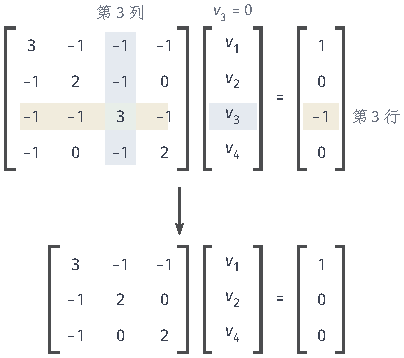
\includegraphics[scale=1]{figures/03-graphs/05-matrices-and-spectra/tikz/electrical-grounded-matrix/figure.pdf}
  \caption{在顶点$3$接地。上方是四点网络的全系统，蓝色竖带标出乘$v_3$的一列，黄色横带标出顶点$3$的方程。约化系统保留顶点$1,2,4$的未知量和守恒式。}
  \label{fig:electrical-grounded-matrix}
\end{BookInlineFigure}

\begin{figure}[!htb]
\centering
\begin{tikzpicture}[x=1mm,y=1mm,>=Stealth,
  vertex/.style={circle,draw=FigureBlue,fill=FigureBlueFill,inner sep=0pt,
    minimum size=5.5mm,line width=.52pt,font=\figurefont\fontsize{8}{10}\selectfont},
  gnd/.style={vertex,fill=FigureBlueFill,draw=FigureBlue,line width=.72pt},
  inject/.style={vertex,fill=FigureYellowFill,draw=FigureYellow,line width=.72pt},
  elabel/.style={font=\figurefont\fontsize{7}{8.5}\selectfont,FigureInk},
  vlabel/.style={font=\figurefont\fontsize{7.5}{9}\selectfont,FigureInk},
  panel/.style={anchor=mid,font=\figurefont\footnotesize}]
  % Left: setup
  \begin{scope}[xshift=0mm]
    \node[inject] (l1) at (0,14) {$1$};
    \node[vertex] (l2) at (14,14) {$2$};
    \node[gnd]    (l3) at (14,0) {$3$};
    \node[vertex] (l4) at (0,0) {$4$};
    \draw[FigureStroke,line width=.45pt] (l1)--(l2) (l2)--(l3) (l3)--(l4) (l4)--(l1) (l1)--(l3);
    \draw[->,FigureYellow,line width=.8pt] (-6,14) -- (l1) node[vlabel,midway,above] {$+1$};
    \draw[->,FigureBlue,line width=.8pt]  (l3) -- (20,0) node[vlabel,midway,above] {$-1$};
    \node[vlabel,below=1mm] at (l3.south) {接地};
    \node[panel] at (7,-8) {(a) 注入与接地};
  \end{scope}
  % Arrow
  \draw[->,FigureStroke,line width=.7pt] (26,7) -- (38,7) node[midway,above,font=\figurefont\fontsize{7}{8.5}\selectfont] {求解};
  % Right: solution
  \begin{scope}[xshift=44mm]
    \node[inject] (r1) at (0,14) {$1$};
    \node[vertex] (r2) at (14,14) {$2$};
    \node[gnd]    (r3) at (14,0) {$3$};
    \node[vertex] (r4) at (0,0) {$4$};
    \draw[FigureStroke,line width=.45pt] (r1)--(r2) (r2)--(r3) (r3)--(r4) (r4)--(r1) (r1)--(r3);
    \node[vlabel,left=1.5mm] at (r1) {$\frac{1}{2}$};
    \node[vlabel,right=1.5mm] at (r2) {$\frac{1}{4}$};
    \node[vlabel,right=1.5mm] at (r3) {$0$};
    \node[vlabel,left=1.5mm] at (r4) {$\frac{1}{4}$};
    % Current arrows
    \draw[->,FigureBlue,line width=.65pt] ([xshift=.5mm,yshift=-1mm]r1.east) -- ([xshift=-.5mm,yshift=-1mm]r2.west) node[elabel,above=.5mm,midway] {$\frac{1}{4}$};
    \draw[->,FigureBlue,line width=.65pt] ([xshift=-1mm,yshift=.5mm]r2.south) -- ([xshift=-1mm,yshift=-.5mm]r3.north) node[elabel,left=.5mm,midway] {$\frac{1}{4}$};
    \draw[->,FigureBlue,line width=.65pt] ([xshift=1mm,yshift=.5mm]r4.north) -- ([xshift=1mm,yshift=-.5mm]r1.south) node[elabel,right=.5mm,midway] {$\frac{1}{4}$};
    \draw[->,FigureBlue,line width=.65pt] ([xshift=.5mm,yshift=1mm]r3.west) -- ([xshift=-.5mm,yshift=1mm]r4.east) node[elabel,below=.5mm,midway] {$\frac{1}{4}$};
    \draw[->,FigureBlue,line width=.85pt] ([xshift=1.5mm,yshift=-1.5mm]r1.south east) -- ([xshift=-1.5mm,yshift=1.5mm]r3.north west) node[elabel,above right=0mm,midway] {$\frac{1}{2}$};
    \node[panel] at (7,-8) {(b) 电势与电流};
  \end{scope}
\end{tikzpicture}
\caption{四点电网络的接地求解。(a) 在顶点$1$注入$1$单位电流（浅黄），在顶点$3$接地（浅蓝）并引出$1$单位。(b) 求解后的电势标在顶点旁，蓝色箭头和数值给出实际电流方向及大小。对角边承载$1/2$的电流，两条外侧支路各承载$1/4$。}
\label{fig:electrical-grounding-overview}
\end{figure}

\begin{figure}[htbp]
  \centering
  \begin{tikzpicture}[
  figure picture,
  terminal/.style={circle,draw=FigureStroke,fill=FigureModelFill,
    minimum size=7mm,inner sep=0pt,line width=.75pt},
  conductor/.style={figure flow},
]
  \node[terminal] (v1) at (-2.3,0) {$1$};
  \node[terminal] (v2) at (0,1.3) {$2$};
  \node[terminal] (v3) at (2.3,0) {$3$};
  \node[terminal] (v4) at (0,-1.3) {$4$};

  \draw[conductor] (v1) -- node[figure edge label,above left] {$1/4$} (v2);
  \draw[conductor] (v2) -- node[figure edge label,above right] {$1/4$} (v3);
  \draw[conductor] (v1) -- node[figure edge label,below left] {$1/4$} (v4);
  \draw[conductor] (v4) -- node[figure edge label,below right] {$1/4$} (v3);
  \draw[conductor] (v1) -- node[figure edge label,above] {$1/2$} (v3);

  \node[left=4pt of v1] {$v_1=1/2$};
  \node[above=4pt of v2] {$v_2=1/4$};
  \node[right=4pt of v3] {$v_3=0$};
  \node[below=4pt of v4] {$v_4=1/4$};
\end{tikzpicture}

  \caption{四点环加对角边的电流分配。各边电导为一，顶点$1$注入一单位电流，顶点$3$接地并引出一单位。节点旁标注电势，边上箭头和数值给出实际电流方向及大小。两条外侧支路各输送$1/4$，中间支路输送$1/2$。}
  \label{fig:electrical-current-split}
\end{figure}

\subsection{一般网络的数值求解}
\label{sec:electrical-numerical-solve}

对于一般的连通电网络，接地后的约化方程组$\overline{\bm L}\,\overline{\bm v} = \overline{\bm b}$是一个$(n-1)$阶对称正定线性方程组，不接地时在正交补子空间$\bm 1^\perp$上求最小范数解$\bm v_{\mathrm{zm}}=\bm L^\dagger\bm b$则是对称半正定相容方程组的求解问题。因此，\BookChapterRef{part:linear-equations-optimization}{卷二第三部分“线性方程与优化”}中建立的各类线性方程组求解方法均可直接应用于电网络求解。

首先是直接分解法（详见\BookChapterRef{chap:direct-linear-solvers}{卷二“线性方程的直接求解”章}），如LU分解、对称正定矩阵的Cholesky分解$\overline{\bm L}=\bm G\bm G^\top$或分块$\bm L\bm D\bm L^\top$分解，在精确算术下通过前代与回代于有限步内求出电势；浮点实现还需控制舍入误差。当图结构与接地点固定而需对多个注入右端$\overline{\bm b}$反复求解时，三角因子可重复使用；但在稀疏图上消去内部顶点$i$会使它的所有邻居两两产生新的非零耦合项（即消元填充现象，见图~\ref{fig:electrical-cholesky-fill-in}），实际存储与计算开销取决于消元顺序下的填充边数量。

其次是定常迭代法（详见\BookChapterRef{sec:ls-stationary-iterations}{卷二“定常迭代法”章}）与行列投影法（详见\BookChapterRef{sec:ls-row-projection}{卷二“行列投影迭代法”章}），如Richardson、Jacobi、Gauss--Seidel、逐次超松弛（SOR/SSOR）或Kaczmarz投影法，仅通过局部邻域电势更新逐步逼近平衡电势，无需改动原图的稀疏结构。

再者是Krylov子空间法与预条件技术（详见\BookChapterRef{chap:krylov-methods}{卷二“Krylov子空间法”章}），如共轭梯度法（CG）、最小残差法（MINRES）与预条件共轭梯度法（PCG）。每步迭代的核心运算只需遍历全部$m$条边计算一次稀疏矩阵向量乘法$\bm x\mapsto\bm L\bm x$（耗时$O(n+m)$）；对条件数为$\kappa=\kappa_2(\bm A)$的正定系统$\bm A\bm x=\bm d$，共轭梯度法第$k$步能量范数误差满足
\begin{equation}
  \lVert\bm e^{(k)}\rVert_{\bm A}
  \leq 2\left(\frac{\sqrt\kappa - 1}{\sqrt\kappa + 1}\right)^k
  \lVert\bm e^{(0)}\rVert_{\bm A}.
  \label{eq:electrical-cg-error}
\end{equation}
至于直接法与各类迭代法在误差控制与总计算成本上的权衡选择，可参见\BookChapterRef{chap:solution-error-regularization}{卷二“求解误差、正则化与方法选择”章}；第~\ref{chap:graph-sparsification}章还将专门讨论如何用图的谱稀疏化构造拉普拉斯预条件子。

\begin{BookInlineFigure}
  \centering
  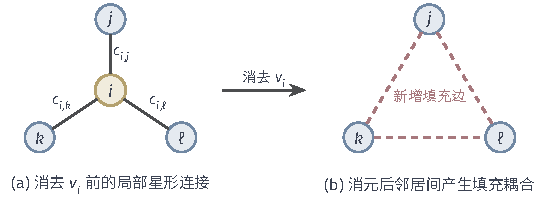
\includegraphics[width=92.385mm]{figures/03-graphs/05-matrices-and-spectra/tikz/electrical-cholesky-fill-in/figure.pdf}
  \caption{稀疏电网络直接消元中的填充现象。（a）消去顶点$i$之前，$i$与三个彼此不相邻的邻居$j,k,\ell$呈星形连接。（b）消去$v_i$后，邻居$j,k,\ell$之间两两产生新的非零耦合项（红色虚线填充边）。}
  \label{fig:electrical-cholesky-fill-in}
\end{BookInlineFigure}

\subsection{树上的线性时间求解}
\label{sec:electrical-tree-solve}

当电网络的正权支撑是一棵树$T=(V,E)$（边数$m=n-1$）时，图中不存在环路；按叶节点到根的顺序消元不会产生填充，任意消元顺序则未必如此。利用树的无环结构，无需显式构造矩阵，只需通过“自底向上求边电流、自顶向下求顶点电势”的两遍树遍历，就能在$O(n)$线性时间内精确解出拉普拉斯方程$\bm L\bm v=\bm b$。

先推导树上边电流与子树注入量的直接关系。任选顶点$q\in V$作为树的根（并令其为接地点$v_q=0$）。对每个非根顶点$i\neq q$，记$p(i)$为其父顶点，并将连接$i$与$p(i)$的唯一树边定向为从子指向父：$e_i\colon i\to p(i)$。删去树边$e_i$会将整棵树恰好切分为两部分：以$i$为根的子树$T_i$，以及包含根$q$的其余部分$V\setminus T_i$。

将子树$T_i$内部所有顶点$u\in T_i$的Kirchhoff电流守恒方程相加：子树内部的每一条边两个端点都在$T_i$内，其电流在尾端贡献正值、在头端贡献负值，正负成对抵消；唯一一条一端在$T_i$内、另一端在$T_i$外（即父顶点$p(i)$）的边界边正是$e_i\colon i\to p(i)$。因此，从$i$流向父顶点$p(i)$的边电流$s_i = f_{i\to p(i)}$必然精确等于整棵子树$T_i$内部的外部注入总和：
\begin{equation}
  s_i = \sum_{u\in T_i} b_u = b_i + \sum_{j\colon p(j) = i} s_j\qquad (i\neq q).
  \label{eq:electrical-subtree-injection}
\end{equation}

有了每条树边上的电流$s_i$后，再沿每条边$i\to p(i)$应用Ohm定律$s_i = c_{i,p(i)}(v_i - v_{p(i)})$，即可由父顶点的电势$v_{p(i)}$直接递推算出子顶点$i$的电势：
\begin{equation}
  v_i = v_{p(i)} + r_{i,p(i)}\,s_i\qquad (i\neq q),
  \label{eq:electrical-tree-voltage}
\end{equation}
其中$r_{i,p(i)} = 1/c_{i,p(i)}$为该树边的电阻。

据此，树上拉普拉斯方程$\bm L\bm v=\bm b$的$O(n)$求解算法完整流程如下（图~\ref{fig:electrical-tree-two-pass}）：

\paragraph{第一阶段：定根与父子序构建}
以接地点$q$为根，从$q$出发作一次广度优先或深度优先搜索，确定每个非根顶点$i\neq q$的父顶点$p(i)$及子节点列表，并按从根到叶的顺序记录遍历序列$(u_1=q, u_2, \ldots, u_n)$（父节点始终排在子节点之前）。

\paragraph{第二阶段：自底向上汇总子树注入求边电流（子节点先于父节点）}
按序列的逆序$u_n, u_{n-1}, \ldots, u_1$（即从叶子向根的自底向上顺序，此时处理顶点$i$时其所有子节点$j$的$s_j$均已算出）依次计算式~\eqref{eq:electrical-subtree-injection}：
\[
  s_i \leftarrow b_i + \sum_{j\colon p(j)=i} s_j.
\]
对叶节点，求和为空，直接有$s_i = b_i$；对内部节点$i\neq q$，算出的$s_i$即为边$i\to p(i)$上的电流。到达根节点$q$时，算出$s_q = \sum_{u\in V}b_u$：若$s_q\neq 0$，则外部注入总和不为零，报告方程组无解并终止；若$s_q = 0$，进入第三阶段。

\paragraph{第三阶段：自顶向下累加压降恢复顶点电势（父节点先于子节点）}
固定根节点电势$v_q \leftarrow 0$。按正序$u_2, \ldots, u_n$（即从根向叶的自顶向下顺序，此时处理顶点$i$时其父电势$v_{p(i)}$已经算出）依次由式~\eqref{eq:electrical-tree-voltage}计算
\[
  v_i \leftarrow v_{p(i)} + r_{i,p(i)}\,s_i.
\]
遍历结束即得全部顶点的唯一接地电势向量$\bm v$与全部树边的电流（若原边参考方向为$p(i)\to i$，只需将该边电流取为$-s_i$）。三个阶段均只对每个顶点和每条树边访问常数次，总时间复杂度和空间复杂度均为$O(n)$。

\begin{BookInlineFigure}
  \centering
  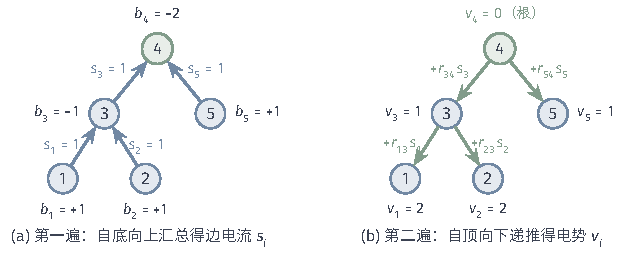
\includegraphics[width=105.174mm]{figures/03-graphs/05-matrices-and-spectra/tikz/electrical-tree-two-pass/figure.pdf}
  \caption{五顶点单位电阻树（以顶点$4$为根，注入$\bm b=(1,1,-1,-2,1)^\top$）上的两遍线性时间求解过程。（a）第一遍自底向上（从叶向根）按$s_i=b_i+\sum_{j:p(j)=i}s_j$汇总子树注入，直接定出每条边指向父节点的电流$s_1=1,s_2=1,s_3=-1+1+1=1,s_5=1$。（b）第二遍自顶向下（从根$v_4=0$向叶）按$v_i=v_{p(i)}+r_{i,p(i)}s_i$逐层累加压降，算出各点电势$v_3=1,v_5=1,v_1=2,v_2=2$。}
  \label{fig:electrical-tree-two-pass}
\end{BookInlineFigure}

以图~\ref{fig:electrical-tree-two-pass}中的五顶点单位电阻树（$r_e=1$）核对算法过程：设根为$4$，顶点$3$和$5$以$4$为父，叶子$1$和$2$以$3$为父，外部注入为$\bm b=(1,1,-1,-2,1)^\top$。

第一遍自底向上：叶子$1,2,5$直接取自身注入，得$s_1=1$、$s_2=1$、$s_5=1$；内部顶点$3$汇总自身注入$b_3=-1$与两个子节点的$s_1,s_2$，得$s_3 = -1 + 1 + 1 = 1$；根$4$处汇总得$s_4 = b_4 + s_3 + s_5 = -2 + 1 + 1 = 0$，守恒条件满足。

第二遍自顶向下：令根电势$v_4 = 0$；第一层子节点电势为$v_3 = v_4 + 1\times s_3 = 1$、$v_5 = v_4 + 1\times s_5 = 1$；第二层叶子电势为$v_1 = v_3 + 1\times s_1 = 2$、$v_2 = v_3 + 1\times s_2 = 2$，即得唯一接地电势解$\bm v=(2,2,1,0,1)^\top$。

\section{能量最小原理}
\label{sec:electrical-minimum-energy}

同样从顶点$1$送入一单位电流、从顶点$3$取出，可以有不同的分法。一种是把整股电流全部交给对角边，沿$1\to3$直走。另一种是让一半走对角边，另一半经过顶点$2$：先从$1$到$2$输送$1/2$，再从$2$到$3$输送$1/2$，对角边也输送$1/2$。两种分法在顶点$1$和$3$的净流出都是$1$和$-1$，在顶点$2$和$4$的净流出都是零——守恒条件满足得一样好。

哪种分法更优？我们比较两者的总耗散。一条边的耗散是电流乘压降。由Ohm定律，电阻为$r_e$的边上，压降为$r_e f_e$，耗散因此等于$r_e f_e^2$。电流翻一倍，耗散变成四倍。全网络的总耗散是各条边的贡献之和：
\begin{equation}
  \mathcal E(\bm f)
  = \sum_{e\in E} r_e f_e^2
  = \bm f^\top \bm C^{-1} \bm f.
  \label{eq:electrical-dissipation}
\end{equation}

四点图的边电阻都为一。全部走对角边时，只有一条边有电流$1$，耗散为$1^2 = 1$。一半走对角边、一半经顶点$2$时，三条边的电流各为$1/2$，耗散为$3 \times (1/2)^2 = 3/4$。分散在更多支路上，耗散反而更低了。

\paragraph{最小耗散定理}

那么在给定注入条件$\bm B\bm f = \bm b$下，哪种分法的耗散最小？答案正是上一节方程给出的实际电流。

\begin{theorem}[Thomson原理]
\label{thm:electrical-thomson}
设网络的边电导为正，各正权连通分量内的注入总量为零。对拉普拉斯方程的任一解$\bm v$，由Ohm定律得到的电流$\bm f_\star = \bm C\bm B^\top \bm v$是满足$\bm B\bm f = \bm b$的唯一最小耗散流。最小耗散为
\begin{equation}
  \mathcal E(\bm f_\star) = \bm b^\top \bm L^\dagger \bm b.
  \label{eq:electrical-minimum-dissipation}
\end{equation}
\end{theorem}

\begin{proof}
取任意另一组守恒流$\bm f$，记它与实际电流的差为$\bm z = \bm f - \bm f_\star$。两者满足同样的注入条件，因此差向量的净流出处处为零：$\bm B\bm z = \bm 0$。按第~\ref{chap:graph-incidence-matrix}章的术语，$\bm z$是一个环流。叠加环流改变各边的流量，但每个顶点的净流出保持原值。

将$\bm f = \bm f_\star + \bm z$代入总耗散并展开：
\[
  \mathcal E(\bm f_\star + \bm z)
  = \mathcal E(\bm f_\star) + \mathcal E(\bm z) + 2\bm f_\star^\top \bm C^{-1}\bm z.
\]
前两项分别是实际电流自身的耗散和附加环流自身的耗散。关键在于交叉项。

交叉项中，$\bm C^{-1}\bm f_\star$的第$e$项是$r_e f_{\star,e}$，也就是该边的压降$v_i - v_j$。所以
\[
  \bm f_\star^\top \bm C^{-1}\bm z
  = (\bm B^\top \bm v)^\top \bm z
  = \bm v^\top \bm B\bm z.
\]
第一个等号把每条边上的电阻乘电流换成电势差，第二个等号用到转置。由于$\bm B\bm z = \bm 0$，这个内积等于零。

直观地说，这是因为每个顶点$i$的贡献是$v_i \times (\bm B\bm z)_i = 0$。环流在每处进出相抵，电势无论取什么值都无法从中提取出功率。

去掉为零的交叉项后，
\begin{equation}
  \mathcal E(\bm f_\star + \bm z)
  = \mathcal E(\bm f_\star) + \mathcal E(\bm z).
  \label{eq:electrical-dissipation-decomposition}
\end{equation}
各边电阻为正，非零环流的耗散严格为正。因此任何不同于$\bm f_\star$的守恒流都有更大的耗散，极小流存在且唯一。

最后用顶点数据表示最小耗散。实际电流的耗散可以改写为
\[
  \mathcal E(\bm f_\star)
  = (\bm B^\top \bm v)^\top \bm C (\bm B^\top \bm v)
  = \bm v^\top \bm L\bm v.
\]
再用$\bm L\bm v = \bm b$，得到$\mathcal E(\bm f_\star) = \bm b^\top \bm v$。每个顶点的贡献是注入量乘电势：注入端电势高，取出端电势低，正注入乘正电势给出正的功率。

若某个分量的电势整体平移$c$，多出来的一项$c \cdot \bm 1^\top \bm b = 0$，所以耗散不依赖电势基准。取各分量内零均值的解$\bm v = \bm L^\dagger \bm b$，便得到式~\eqref{eq:electrical-minimum-dissipation}。
\end{proof}

这个结论称为\term{Thomson原理}（Thomson's principle）。

\paragraph{算例验证}

回到四点图的实际电流。四条环边各载$1/4$，耗散各为$(1/4)^2 = 1/16$。对角边载$1/2$，耗散为$(1/2)^2 = 1/4$。总耗散为$4 \times 1/16 + 1/4 = 1/2$。

现在取第~\ref{sec:incidence-cycle-space}节的基本环$\bm c_1$，它沿$1\to2\to3\to4\to1$的四条环边各送$1/4$个单位。叠加之后，看各条边的变化：

边$12$和$23$上原来各有$1/4$的电流，加上$1/4$变成$1/2$。

边$34$和$41$上原来各有$-1/4$的电流（实际从$4$流向$3$和从$1$流向$4$），加上$1/4$后恰好抵消为零。

对角边不在这个环上，仍然流过$1/2$。

这恰好就是本节开头的第二种分法：一半走对角边，一半经顶点$2$。由式~\eqref{eq:electrical-dissipation-decomposition}，附加环流使耗散增加$4 \times (1/4)^2 = 1/4$。已知实际耗散$1/2$，加上这一项得到$3/4$，与直接计算一致。

图~\ref{fig:electrical-distribution-dissipation}并排画出三种分流。(a)所有电流只走一条边，耗散为$1$。(b)分到两条路径后耗散降至$3/4$。(c)是网络自行选择的实际分流，耗散最低，为$1/2$。

\begin{BookInlineFigure}
  \centering
  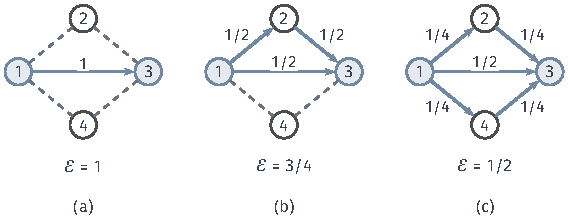
\includegraphics[scale=1]{figures/03-graphs/05-matrices-and-spectra/tikz/electrical-distribution-dissipation/figure.pdf}
  \caption{同一单位注入下的三种分流。顶点$1$注入一单位电流，顶点$3$引出一单位，各边电阻都为一。箭头和数值给出有流量的边，虚线为零电流的边。(a)~只走对角边，(b)~平分到对角边和上路，(c)~网络的实际分流。}
  \label{fig:electrical-distribution-dissipation}
\end{BookInlineFigure}

\paragraph{与最小费用流的比较}

第~\ref{chap:min-cost-flow}章的最小费用流也在守恒条件下选流量，但目标函数是线性的，通常还有容量约束。这里的耗散是严格凸的二次函数，不存在容量限制，边流可以取任意实数。正因为严格凸，极小点唯一——不需要另外检查是否有多个最优解。即使注入量为整数，最优的边流量也可能是分数，如本例中的$1/4$和$1/2$。

\section{有效电阻}
\label{sec:graph-effective-resistance}

从外部观察一个电网络时，如果只在两个选定端点$a$和$b$之间接入一单位电流并测量这两点之间的电势差，网络内部复杂的串并联与环路分流就被浓缩为一个标量——两点之间的有效电阻。本节依次介绍有效电阻的定义与三种等价表达、不同复杂度网络上有效电阻的精确计算方法、大规模网络上有效电阻的三种近似计算方法，以及有效电阻作为图上距离度量的基本性质。

\subsection{有效电阻的定义}
\label{sec:electrical-resistance-definition}

单条电阻为$r$的边在通过$1$单位电流时产生压降$r$。把这一测量方式推广到整张网络中的任意一对顶点$a,b$，就得到有效电阻的定义。

\begin{definition}[有效电阻]
\label{def:graph-effective-resistance}
设$a,b$是同一正权连通分量中的两个不同顶点。取单位偶极注入向量$\bm b_{a,b} = \bm e_a - \bm e_b$（即在顶点$a$注入$1$单位电流、从顶点$b$引出$1$单位电流，其余顶点注入为零）。设$\bm v\in\mathbb R^n$为拉普拉斯方程$\bm L\bm v = \bm b_{a,b}$的任一电势解，定义顶点$a$与$b$之间的\term{有效电阻}（effective resistance）为
\begin{equation}
  R_{a,b} = v_a - v_b.
  \label{eq:electrical-resistance-definition}
\end{equation}
此外，约定同一点的有效电阻为$R_{a,a} = 0$；若$a,b$分属不同的正权连通分量，约定$R_{a,b} = +\infty$。
\end{definition}

由定理~\ref{thm:electrical-laplacian-solvability}(2)，不同电势解在每个正权连通分量上分别相差一个常数；对包含$a,b$的分量记这一常数为$c$，相减后$(v_a+c)-(v_b+c)=v_a-v_b$，故定义~\ref{def:graph-effective-resistance}完全不依赖接地点的选取。若将注入电流从$1$单位改为任意$I$单位（即右端取$I\bm b_{a,b}$），由方程的线性性，两端电势差变为$v_a - v_b = I\cdot R_{a,b}$，说明整张网络对外部端点$a,b$的端口响应完全等价于在$a,b$之间单独连接一个阻值为$R_{a,b}$的电阻器。

除了定义式~\eqref{eq:electrical-resistance-definition}外，有效电阻还有两种常用的等价代数与变分表达：

第一种是\emph{伪逆二次型表达}。在连通分量上取零均值电势解$\bm v = \bm L^\dagger \bm b_{a,b}$，由于$v_a - v_b = (\bm e_a - \bm e_b)^\top\bm v = \bm b_{a,b}^\top\bm v$，代入即得
\begin{equation}
  R_{a,b}
  = \bm b_{a,b}^\top \bm L^\dagger \bm b_{a,b}
  = (\bm e_a - \bm e_b)^\top \bm L^\dagger (\bm e_a - \bm e_b)
  = L^\dagger_{a,a} + L^\dagger_{b,b} - 2L^\dagger_{a,b}.
  \label{eq:electrical-resistance-pseudoinverse}
\end{equation}

第二种是\emph{Thomson最小耗散表达}。在定理~\ref{thm:electrical-thomson}的式~\eqref{eq:electrical-minimum-dissipation}中取$\bm b = \bm b_{a,b} = \bm e_a - \bm e_b$，最小总耗散为$\bm b_{a,b}^\top\bm L^\dagger\bm b_{a,b} = v_a - v_b = R_{a,b}$，因此有效电阻恰好等于从$a$向$b$输送$1$单位守恒流所需的最小总耗散：
\begin{equation}
  R_{a,b} = \min_{\bm B\bm f = \bm e_a - \bm e_b} \bm f^\top \bm C^{-1} \bm f.
  \label{eq:electrical-resistance-energy}
\end{equation}
式~\eqref{eq:electrical-resistance-pseudoinverse}便于通过线性代数直接计算单对或多对顶点的有效电阻；式~\eqref{eq:electrical-resistance-energy}则便于分析网络结构变化（如添边或增大电导）对有效电阻的单调影响。

\subsection{有效电阻的计算}
\label{sec:electrical-series-parallel}

针对结构复杂度不同的电网络，可以按由简入繁的顺序选用三种精确计算方法：对串并联简单结构直接作局部归约；对含桥式结构的小规模网络考虑星-三角（$\text{Y--}\Delta$）变换；对一般中等规模网络直接求解接地拉普拉斯线性方程组。

\subsubsection{简单结构：串联、并联与悬空支路}
\label{sec:electrical-simple-reductions}

当网络局部只包含串联路径、并联重边或无源悬空支路时，可以逐步将局部子网替换为单条等效边，同时保持端口的电势差与电流关系不变。

\paragraph{串联归约}
设两条边$e_1=\{u,w\}$与$e_2=\{w,v\}$在内部顶点$w$处首尾相接，且中间顶点$w$的度数为$2$、没有外部电流注入（$b_w=0$）。此时Kirchhoff电流定律要求流过两条边的电流大小完全相同，记为$I$。两段边上的压降分别为$I r_1$与$I r_2$，从$u$到$v$的总压降为$I(r_1 + r_2)$，因此可将两条串联边合并为一条连接$u,v$的等效边，其等效电阻等于两段电阻之和：
\begin{equation}
  r_{\mathrm{series}} = r_1 + r_2, \qquad
  c_{\mathrm{series}} = \frac{c_1 c_2}{c_1 + c_2}.
  \label{eq:electrical-series}
\end{equation}
需要注意，若中间顶点$w$还连接着第三条边或有外部电流注入，流过两段的电流一般不同，不能直接套用串联公式。

\paragraph{并联归约}
设连接同一对端点$u,v$的多条支路具有电导$c_1,c_2,\ldots,c_k$。由于它们共用相同的两端压降$\Delta v = v_u - v_v$，第$i$条支路流过的电流为$c_i\Delta v$，总电流为$\bigl(\sum_i c_i\bigr)\Delta v$。因此可将多条并联支路合并为一条等效边，其等效电导等于各支路电导之和（等效电阻为总电导的倒数）：
\begin{equation}
  c_{\mathrm{parallel}} = \sum_i c_i, \qquad
  r_{\mathrm{parallel}} = \left(\sum_i \frac{1}{r_i}\right)^{-1}.
  \label{eq:electrical-parallel}
\end{equation}
此外，若网络中存在不包含查询端点$a,b$的悬空叶节点（度为$1$且无外部注入），由电流守恒知该悬空边上的电流必为零，可直接将其删去而不影响$R_{a,b}$。

\begin{BookInlineFigure}
  \centering
  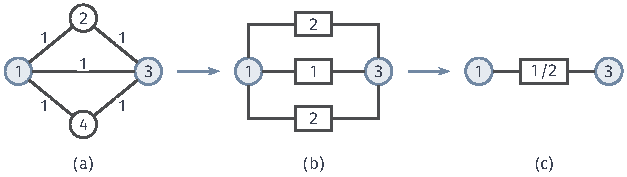
\includegraphics[scale=1]{figures/03-graphs/05-matrices-and-spectra/tikz/electrical-series-parallel-reduction/figure.pdf}
  \caption{四点网络在端点$1,3$之间的串并联简化。数字是边或支路的电阻。(a)~五条单位电阻边，(b)~分别合并经过顶点$2$和顶点$4$的两组串联边，得到阻值为$2,1,2$的三条并联支路，(c)~再合并为阻值$1/2$的单条边。}
  \label{fig:electrical-series-parallel-reduction}
\end{BookInlineFigure}

以四点五边单位电阻图（每条边$r_e=1$）计算$R_{1,3}$为例（图~\ref{fig:electrical-series-parallel-reduction}）。当查询端点为$1$和$3$时，中间顶点$2$和$4$的度数均为$2$且无外部注入：

第一步，作串联归约（图~\ref{fig:electrical-series-parallel-reduction}(b)）。经过顶点$2$的两条边$12,23$串联，合并为连接$1,3$、阻值为$1+1=2$（电导$1/2$）的上支路；经过顶点$4$的两条边$14,43$同样串联，合并为阻值为$1+1=2$（电导$1/2$）的下支路。

第二步，作并联归约（图~\ref{fig:electrical-series-parallel-reduction}(c)）。现在端点$1,3$之间共有三条并联支路，电阻分别为$2,1,2$，电导分别为$1/2,1,1/2$。将三者电导相加得总电导$c_{\mathrm{parallel}} = 1/2 + 1 + 1/2 = 2$，取倒数立得
\[
  R_{1,3} = \frac{1}{1/2 + 1 + 1/2} = \frac{1}{2},
\]
与例~\ref{ex:electrical-four-vertex-network}通过解方程算出的$v_1 - v_3 = 1/2 - 0 = 1/2$完全一致。

\subsubsection{小规模桥式结构：星-三角变换}
\label{sec:electrical-wye-delta}

单纯依靠串联和并联归约并不能化简所有双端网络。例如在四点环加对角边$13$的五边图上，以$2,4$为查询端点时，两个内部顶点$1,3$的度数都为$3$，既没有可消去的二度无源顶点，也没有平行重边。这是一个桥式结构；若各臂阻值恰好平衡，还可另用对称性化简，但一般边权下不能作此假设。

对于度为$3$的内部接点，可用\emph{星-三角变换}（$\text{Y--}\Delta$ transformation）：把以无源顶点$w$为中心的三条星形支路替换为三个外围顶点之间的三角形支路，或反向操作，同时保持端口电势与电流关系（图~\ref{fig:electrical-wye-delta-bridge}(a)）。下文选取仍可串并联化简的$R_{1,2}$作为计算示例，以便交叉核验变换结果。

\begin{theorem}[星-三角（$\text{Y--}\Delta$）等效变换]
\label{thm:electrical-wye-delta}
设中心顶点$w$不接入外部电流（$b_w=0$），且仅与三个外围顶点$u_1,u_2,u_3$相连，三条星形支路的电导分别为$c_1,c_2,c_3>0$（对应电阻为$r_1,r_2,r_3$）。消去中心顶点$w$后，该星形子网对$u_1,u_2,u_3$的端口电势与电流关系，完全等价于在$u_1,u_2,u_3$之间两两连接一条三角形边，其中连接$u_i$与$u_j$（$1\leq i<j\leq 3$，记第三个下标为$k$）的等效电导$c_{i,j}$与等效电阻$r_{i,j}$分别为
\begin{equation}
  c_{i,j} = \frac{c_i c_j}{c_1 + c_2 + c_3}, \qquad
  r_{i,j} = \frac{r_1 r_2 + r_2 r_3 + r_3 r_1}{r_k}.
  \label{eq:electrical-y-to-delta}
\end{equation}
反之，若已知$u_1,u_2,u_3$之间的三角形边电阻为$r_{1,2},r_{2,3},r_{3,1}>0$，将其等价变换为以新增无源顶点$w$为中心的星形支路（$\Delta\to\text{Y}$变换）时，连接$u_i$与$w$的星形支路电阻为
\begin{equation}
  r_i = \frac{r_{i,j}\,r_{i,k}}{r_{1,2} + r_{2,3} + r_{3,1}} \qquad (\{i,j,k\}=\{1,2,3\}).
  \label{eq:electrical-delta-to-y}
\end{equation}
\end{theorem}

\begin{proof}
在星形网络中，中心顶点$w$无外部注入（$b_w=0$），其Kirchhoff电流守恒方程为
\[
  (c_1 + c_2 + c_3)v_w - (c_1 v_1 + c_2 v_2 + c_3 v_3) = 0,
\]
解出中心电势为外围三点电势的加权平均：
\[
  v_w = \frac{c_1 v_1 + c_2 v_2 + c_3 v_3}{c_1 + c_2 + c_3}.
\]

将$v_w$代入外围顶点$u_1$从星形子网流出的电流$I_1 = c_1(v_1 - v_w)$，通分整理得
\[
  \begin{aligned}
    I_1
    &= c_1\left(v_1 - \frac{c_1 v_1 + c_2 v_2 + c_3 v_3}{c_1 + c_2 + c_3}\right)\\
    &= \frac{c_1 c_2}{c_1 + c_2 + c_3}(v_1 - v_2) + \frac{c_1 c_3}{c_1 + c_2 + c_3}(v_1 - v_3).
  \end{aligned}
\]
对$u_2$和$u_3$同理。这恰与在$u_i,u_j$之间连接电导为$c_{i,j} = \frac{c_i c_j}{c_1+c_2+c_3}$的三角形边所产生的端口电流完全相同。将$c_i = 1/r_i$代入$r_{i,j}=1/c_{i,j}$并上下同乘$r_1 r_2 r_3$，即得式~\eqref{eq:electrical-y-to-delta}的第二式；求解式~\eqref{eq:electrical-y-to-delta}关于$r_1,r_2,r_3$的代数反演即得$\Delta\to\text{Y}$公式~\eqref{eq:electrical-delta-to-y}。
\end{proof}

\begin{BookInlineFigure}
  \centering
  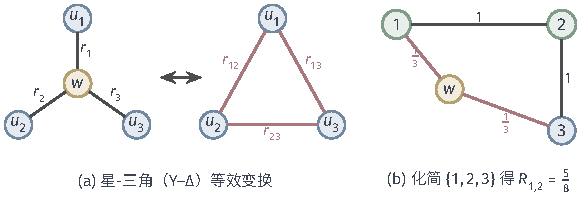
\includegraphics[width=98.591mm]{figures/03-graphs/05-matrices-and-spectra/tikz/electrical-wye-delta-bridge/figure.pdf}
  \caption{星-三角（$\text{Y--}\Delta$）变换及其在桥式结构化简中的应用。（a）无源中心顶点$w$的星形三支路与外围三角形三支路相互等效。（b）计算四点五边图的$R_{1,2}$时，将左下三角形$\{1,3,4\}$通过$\Delta\to\text{Y}$变换化为中心顶点$w$的星形（有效支路电阻为$1/3$），再由串并联算出$R_{1,2}=5/8$。}
  \label{fig:electrical-wye-delta-bridge}
\end{BookInlineFigure}

下面在四点五边单位电阻图上演示如何用星-三角变换求出$R_{1,2}$（图~\ref{fig:electrical-wye-delta-bridge}(b)）。在图$\mathcal G$中，顶点$1,2,3$构成右上三角形，顶点$1,3,4$构成左下三角形：

第一步，对左下角的单位电阻三角形$\{1,3,4\}$（三条边电阻均为$1$）施行$\Delta\to\text{Y}$变换~\eqref{eq:electrical-delta-to-y}。引入星形中心$w$替换该三角形后，连接$1,3,4$的三条星形支路电阻均为
\[
  r_1 = r_3 = r_4 = \frac{1\times 1}{1 + 1 + 1} = \frac{1}{3}.
\]
由于顶点$4$不是查询端点（无外部注入），变换后悬挂在$w$上的支路$w\!-\!4$成为无源悬空叶边，电流为零，直接删去（见图~\ref{fig:electrical-wye-delta-bridge}(b)）。

第二步，对剩余的串并联支路直接求值。在图~\ref{fig:electrical-wye-delta-bridge}(b)中，从端点$1$到端点$2$现在只剩两条并联支路：一条是上方的直接边$1\!-\!2$（电阻为$1$）；另一条依次经过$1\to w\to 3\to 2$，由三段串联组成，总电阻为
\[
  r_{1\to w\to 3\to 2} = \frac{1}{3} + \frac{1}{3} + 1 = \frac{5}{3}.
\]
将阻值为$1$和$5/3$的两条支路并联，立得
\[
  R_{1,2} = \frac{1 \times \frac53}{1 + \frac53} = \frac{5}{8}.
\]

\subsubsection{中等规模网络：求解拉普拉斯方程}
\label{sec:electrical-medium-laplacian-solve}

当网络规模达到数十至数万个顶点、内部包含大量交错环路时，手工寻找星-三角变换和串并联归约不再现实。此时最通用、系统的计算方法是直接回到定义~\ref{def:graph-effective-resistance}：固定端点$b$接地（令$v_b = 0$），在端点$a$注入$1$单位电流，求解$(n-1)\times(n-1)$对称正定线性方程组
\[
  \overline{\bm L}\,\overline{\bm v} = \overline{\bm e}_a,
\]
解出电势后直接读取顶点$a$处的电势值，即有$R_{a,b} = v_a - v_b = v_a$。若需要查询多对顶点之间的有效电阻，可先对$\overline{\bm L}$作一次Cholesky分解（或求出伪逆$\bm L^\dagger$），再利用式~\eqref{eq:electrical-resistance-pseudoinverse}计算$R_{a,b} = L^\dagger_{a,a} + L^\dagger_{b,b} - 2L^\dagger_{a,b}$。

下面用求解拉普拉斯方程的方法重新计算四点五边单位电阻图上的$R_{1,2}$（图~\ref{fig:electrical-r12-potential-flow}），与上一小节的星-三角化简结果核对。设从顶点$1$注入$1$单位电流、从顶点$2$引出$1$单位电流，令顶点$2$接地（$v_2 = 0$）：

第一步，利用无源顶点$4$的守恒方程消去$v_4$。顶点$4$无外部注入，连接邻居$1$和$3$，度为$2$，故
\[
  2v_4 - v_1 - v_3 = 0 \quad\Longrightarrow\quad v_4 = \frac{v_1 + v_3}{2}.
\]

第二步，利用无源顶点$3$的守恒方程求出$v_3$与$v_1$的比例关系。顶点$3$无外部注入，连接邻居$1,2,4$，度为$3$，故
\[
  3v_3 - v_1 - v_2 - v_4 = 0.
\]
将$v_2 = 0$和$v_4 = (v_1 + v_3)/2$代入上式，化简得$5v_3 = 3v_1$，即
\[
  v_3 = \frac{3}{5}v_1, \qquad v_4 = \frac{1}{2}\Bigl(v_1 + \frac{3}{5}v_1\Bigr) = \frac{4}{5}v_1.
\]

第三步，代入注入端顶点$1$的守恒方程解出$v_1$。顶点$1$连接邻居$2,3,4$，度为$3$，外部注入为$1$，故
\[
  3v_1 - v_2 - v_3 - v_4 = 1.
\]
代入$v_2 = 0$、$v_3 = \frac35 v_1$、$v_4 = \frac45 v_1$，得
\[
  3v_1 - 0 - \frac{3}{5}v_1 - \frac{4}{5}v_1 = \frac{8}{5}v_1 = 1
  \quad\Longrightarrow\quad v_1 = \frac{5}{8}.
\]
由此得到全部顶点的接地电势向量为
\[
  \bm v = \Bigl(\frac{5}{8}, \; 0, \; \frac{3}{8}, \; \frac{1}{2}\Bigr)^\top,
\]
两端有效电阻为$R_{1,2} = v_1 - v_2 = 5/8$，与星-三角变换算出的结果完全一致。

\begin{BookInlineFigure}
  \centering
  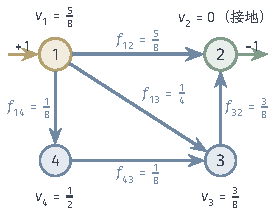
\includegraphics[width=46.718mm]{figures/03-graphs/05-matrices-and-spectra/tikz/electrical-r12-potential-flow/figure.pdf}
  \caption{在四点单位电阻网络中求解$\bm L\bm v=\bm e_1-\bm e_2$（令$v_2=0$接地）计算有效电阻$R_{1,2}=5/8$。顶点旁标注电势值，边上箭头与数字标出五条边的实际分流大小：直接边$1\to 2$承载$5/8$，经由$1\to 3\to 2$和$1\to 4\to 3\to 2$的旁路合流$1/4+1/8=3/8$注入终点$2$。}
  \label{fig:electrical-r12-potential-flow}
\end{BookInlineFigure}

对比$R_{1,2} = 5/8$与$R_{1,3} = 1/2$可以发现：虽然顶点对$(1,2)$和$(1,3)$之间都有一条单位电阻的边直接相连，但$(1,3)$之间有两条对称的二步旁路分担电流，而$(1,2)$之间的旁路需要绕行更远的路径，因此$R_{1,2} > R_{1,3}$。有效电阻综合反映了整张网络在两点之间提供的全体并行通路容量，而不仅仅是直接相连边的电阻。

\subsection{有效电阻的近似计算}
\label{sec:electrical-approximate-resistance}

在包含百万级顶点和边的大规模图（例如社交网络、道路网或第~\ref{chap:graph-sparsification}章的图稀疏化问题，其中需要求出全部$m$条边两端点的有效电阻）上，若直接按定义对每条边求解一次拉普拉斯线性系统，总共需要求解$m$次方程。若每次求解的成本为$T_{\mathrm{solve}}$，这部分总成本为$O(mT_{\mathrm{solve}})$，因所用求解器、精度和预处理复用方式而异。为此，本小节介绍大规模图上批量或快速近似计算有效电阻的三种常见方法：欧氏嵌入与随机投影降维法、谱展开与低频主模态截断法，以及基于随机游走与生成树的蒙特卡洛采样法。

\subsubsection{欧氏嵌入与随机投影降维}
\label{sec:electrical-resistance-embedding}
\label{sec:electrical-resistance-jl}
\label{sec:electrical-resistance-solver-error}

第一种方法是Spielman与Srivastava提出的随机投影法\scite{spielman2011graph}，它将全部点对的有效电阻转化为低维欧氏空间中的两点距离平方，使全图所有边的有效电阻只需通过求解$k=O(\varepsilon^{-2}\log n)$个拉普拉斯线性系统即可在高概率下获得$(1\pm\varepsilon)$相对精度的批量估计，前提是线性求解误差也得到控制。该方法分三步实现：

\paragraph{第一步：精确欧氏嵌入}
设网络连通。从顶点$a$向$b$注入$1$单位电流时，零均值电势解为$\bm u = \bm L^\dagger \bm b_{a,b}$，每条边$e$上的耗散为$c_e\bigl((\bm B^\top\bm u)_e\bigr)^2 = \bigl((\bm C^{1/2}\bm B^\top\bm L^\dagger\bm b_{a,b})_e\bigr)^2$。将“求零均值电势$\bm L^\dagger$—取沿边差分$\bm B^\top$—按$\sqrt{c_e}$缩放$\bm C^{1/2}$”合成为一个$m\times n$矩阵：
\begin{equation}
  \bm Z = \bm C^{1/2} \bm B^\top \bm L^\dagger \in \mathbb R^{m \times n}.
  \label{eq:electrical-resistance-embedding}
\end{equation}
矩阵$\bm Z$的第$a$列$\bm Z\bm e_a\in\mathbb R^m$即为顶点$a$的$m$维精确嵌入坐标。利用$\bm L=\bm B\bm C\bm B^\top$以及伪逆恒等式$\bm L^\dagger\bm L\bm L^\dagger=\bm L^\dagger$，有
\[
  \bm Z^\top \bm Z
  = \bm L^\dagger \bm B\bm C \bm B^\top \bm L^\dagger
  = \bm L^\dagger \bm L \bm L^\dagger
  = \bm L^\dagger.
\]
因此，任意两个顶点$a,b$之间的有效电阻精确等于它们在$\bm Z$中对应坐标列之差的欧氏长度平方：
\[
  \lVert \bm Z(\bm e_a-\bm e_b) \rVert_2^2
  = \bm b_{a,b}^\top \bm Z^\top \bm Z\bm b_{a,b}
  = \bm b_{a,b}^\top \bm L^\dagger \bm b_{a,b}
  = R_{a,b}.
\]

在四点单位权图上核对：从$1$到$3$单位注入的零均值电势为$(1/4, 0, -1/4, 0)^\top$，沿五条边取差得
\[
  \bm Z(\bm e_1 - \bm e_3) = (1/4, \; 1/4, \; -1/4, \; -1/4, \; 1/2)^\top,
\]
五项平方和为$4\times(1/4)^2+(1/2)^2=1/2=R_{1,3}$；同理，对顶点$1,2$，精确列差向量为
\[
  \bm Z(\bm e_1 - \bm e_2) = (5/8, \; -3/8, \; -1/8, \; -1/8, \; 1/4)^\top,
\]
其欧氏长度平方为$25/64+9/64+1/64+1/64+4/64=40/64=5/8=R_{1,2}$。

\paragraph{第二步：随机投影降维与$k$次线性求解}
由于$m$维嵌入矩阵$\bm Z\in\mathbb R^{m\times n}$维数过高，引入一个元素独立同分布于$\mathcal N(0,1/k)$（或$\pm 1/\sqrt{k}$ Rademacher分布）的$k\times m$随机投影矩阵$\bm Q \in \mathbb R^{k \times m}$（$k\ll m$），将所有顶点的坐标列线性压缩为$k\times n$低维坐标矩阵$\bm Y = \bm Q\bm Z$，并用低维坐标差的欧氏长度平方估计有效电阻：
\[
  \widehat R_{a,b} = \lVert \bm Y(\bm e_a - \bm e_b) \rVert_2^2.
\]

计算$\bm Y=\bm Q\bm Z$无需先算出$\bm L^\dagger$或$\bm Z$。记$\bm q_j^\top\in\mathbb R^{1\times m}$为$\bm Q$的第$j$行（$j=1,\ldots,k$），先计算零和右端向量$\bm d_j = \bm B\bm C^{1/2} \bm q_j\in\bm 1^\perp$，然后求解拉普拉斯方程并取零均值解：
\begin{equation}
  \bm L\bm y_j = \bm d_j, \qquad \bm 1^\top \bm y_j = 0.
  \label{eq:electrical-projection-systems}
\end{equation}
由于$\bm y_j = \bm L^\dagger \bm d_j=\bm L^\dagger\bm B\bm C^{1/2}\bm q_j$且$\bm L^\dagger$对称，转置后即得$\bm y_j^\top = \bm q_j^\top \bm C^{1/2} \bm B^\top \bm L^\dagger = \bm q_j^\top \bm Z$，这正是$\bm Y$的第$j$行。因此，只需对$k$个随机右端各求解一次拉普拉斯系统即可得到全部顶点的$k$维坐标$\bm Y$，此后查询任意一对顶点的有效电阻仅需$O(k)$时间。

以四点单位权图演示$k = 3$的投影计算过程（图~\ref{fig:electrical-resistance-coordinate-projection}）。使用随机数种子\texttt{random.Random(17)}按行生成标准正态随机数并除以$\sqrt{3}$得到$3\times 5$矩阵$\bm Q$，其第一行为$\bm q_1^\top\approx(-1.0368, -0.1441, 0.4628, -0.1173, 0.0910)$；左乘$\bm B\bm C^{1/2}$得$\bm d_1 \approx (-0.8284, 0.8926, 0.5159, -0.5801)^\top$，解出零均值电势即得$\bm Y$的第一行$\bm y_1^\top \approx (-0.2071, 0.4073, 0.1290, -0.3291)$。同样解出第二、第三行后，取$\bm Y$中第$1$列与第$3$列之差的平方和即得估计值$\widehat R_{1,3}\approx 0.3680$，第$1$列与第$2$列之差的平方和给出$\widehat R_{1,2}\approx 0.8263$。

\begin{BookInlineFigure}
  \centering
  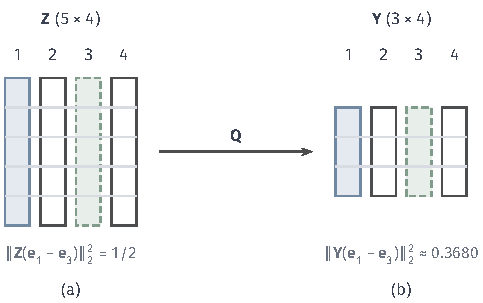
\includegraphics[scale=1]{figures/03-graphs/05-matrices-and-spectra/tikz/electrical-resistance-coordinate-projection/figure.pdf}
  \caption{用两列坐标的欧氏距离平方查询四点图中顶点$1,3$之间的有效电阻。蓝色实框和绿色虚框分别标出顶点$1$和$3$的坐标列。(a)~五维精确坐标$\bm Z$给出$R_{1,3}=1/2$。(b)~左乘随机矩阵$\bm Q$压缩为三维坐标$\bm Y=\bm Q\bm Z$后取列差平方和。}
  \label{fig:electrical-resistance-coordinate-projection}
\end{BookInlineFigure}

下面的定理利用\term{Johnson--Lindenstrauss引理}（Johnson--Lindenstrauss lemma）证明，只需取$k=O(\varepsilon^{-2}\log n)$，就能以高概率同时保证全图所有顶点对的相对误差不超过$\varepsilon$。

\begin{theorem}[高斯投影保留电阻距离]
\label{thm:electrical-jl-resistance}
设$n \geq 2$且正权网络连通，给定相对误差参数$0 < \varepsilon < 1$与失败概率上限$0 < \delta < 1$。令$\bm Q\in\mathbb R^{k\times m}$的元素独立同分布于均值为$0$、方差为$1/k$的正态分布$\mathcal N(0,1/k)$。若投影维数满足
\begin{equation}
  k \geq \frac{8}{\varepsilon^2}\log\frac{n(n-1)}{\delta},
  \label{eq:electrical-projection-dimension}
\end{equation}
则以至少$1 - \delta$的概率，所有顶点对$a,b\in V$同时满足
\begin{equation}
  (1 - \varepsilon)\,R_{a,b}
  \leq \lVert \bm Q\bm Z(\bm e_a - \bm e_b) \rVert_2^2
  \leq (1 + \varepsilon)\,R_{a,b}.
  \label{eq:electrical-projection-guarantee}
\end{equation}
\end{theorem}

\begin{proof}
第一步，分析单个固定非零向量$\bm z\in\mathbb R^m$投影后的分布。由于$\bm Q$的各行独立且元素服从$\mathcal N(0,1/k)$，$\bm Q\bm z$的$k$个分量相互独立且均服从$\mathcal N(0,\lVert\bm z\rVert_2^2/k)$。将各分量除以标准差$\lVert\bm z\rVert_2/\sqrt{k}$后求平方和，所得随机变量
\[
  X = \frac{k\,\lVert\bm Q\bm z\rVert_2^2}{\lVert\bm z\rVert_2^2}=\sum_{j=1}^k \xi_j^2\qquad\bigl(\xi_j\stackrel{\mathrm{i.i.d.}}{\sim}\mathcal N(0,1)\bigr)
\]
服从自由度为$k$的卡方分布，其矩母函数为$\mathbb E[\exp(tX)] = (1 - 2t)^{-k/2}$（$t<1/2$）。

第二步，用Chernoff界估计上下尾概率。对上尾事件$X \geq k(1 + \varepsilon)$，取$t = \varepsilon/[2(1 + \varepsilon)]\in(0,1/2)$应用Markov不等式，得
\[
  \mathbb P\bigl(X \geq k(1 + \varepsilon)\bigr)
  \leq \exp\bigl(-tk(1 + \varepsilon)\bigr)\,(1 - 2t)^{-k/2}
  = \exp\!\left(-\frac{k}{2}\bigl(\varepsilon - \log(1 + \varepsilon)\bigr)\right).
\]
对下尾事件$X \leq k(1 - \varepsilon)$，取$t = -\varepsilon/[2(1 - \varepsilon)] < 0$应用Markov不等式，得
\[
  \mathbb P\bigl(X \leq k(1 - \varepsilon)\bigr)
  \leq \exp\!\left(-\frac{k}{2}\bigl(-\varepsilon - \log(1 - \varepsilon)\bigr)\right).
\]
对$0 < \varepsilon < 1$，利用不等式$\varepsilon-\log(1+\varepsilon)\geq\varepsilon^2/4$和$-\varepsilon-\log(1-\varepsilon)\geq\varepsilon^2/2>\varepsilon^2/4$，合并上下尾可知单个向量$\bm z$的投影长度平方偏离$(1 \pm \varepsilon)\lVert\bm z\rVert_2^2$的概率至多为$2\exp(-k\varepsilon^2/8)$。

第三步，对全部顶点对应用联合界。图中不同顶点的无序对$\{a,b\}$共有$\binom{n}{2}=n(n-1)/2$对，每对对应$\bm z=\bm Z(\bm e_a - \bm e_b)$（长度平方为$R_{a,b}$）。由布尔不等式，至少有一对超出式~\eqref{eq:electrical-projection-guarantee}的概率至多为
\[
  \frac{n(n-1)}{2}\cdot 2\exp\!\left(-\frac{k\varepsilon^2}{8}\right)=n(n-1)\exp\!\left(-\frac{k\varepsilon^2}{8}\right).
\]
当$k$满足式~\eqref{eq:electrical-projection-dimension}时，该概率上界不超过$\delta$。
\end{proof}

\paragraph{第三步：迭代求解的误差控制}
用共轭梯度法近似求解式~\eqref{eq:electrical-projection-systems}的$k$个方程时，设第$j$个方程的近似零均值解为$\widetilde{\bm y}_j$，误差为$\bm h_j = \widetilde{\bm y}_j - \bm y_j$。记单位注入的精确电势为$\bm u = \bm L^\dagger \bm b_{a,b}$，由$\bm L\bm u = \bm b_{a,b}$及能量内积的Cauchy--Schwarz不等式，第$j$行坐标差的误差满足
\[
  |\bm h_j^\top \bm b_{a,b}|
  = |\bm h_j^\top \bm L\bm u|
  \leq \lVert\bm h_j\rVert_{\bm L}\,\lVert\bm u\rVert_{\bm L}
  = \lVert\bm h_j\rVert_{\bm L}\,\sqrt{R_{a,b}}.
\]
若将全部$k$次求解的总能量误差控制在$\sum_{j=1}^k \lVert\bm h_j\rVert_{\bm L}^2 \leq \eta^2$以内，则$\lVert(\widetilde{\bm Y}-\bm Y)\bm b_{a,b}\rVert_2\leq\eta\sqrt{R_{a,b}}$。结合式~\eqref{eq:electrical-projection-guarantee}与三角不等式，对$a\ne b$，最终估计值$\widehat R_{a,b} = \lVert \widetilde{\bm Y}\bm b_{a,b}\rVert_2^2$满足
\begin{equation}
  \max\{0, \sqrt{1-\varepsilon} - \eta\}
  \leq \sqrt{\frac{\widehat R_{a,b}}{R_{a,b}}}
  \leq \sqrt{1+\varepsilon} + \eta.
  \label{eq:electrical-resistance-total-error}
\end{equation}

\subsubsection{谱展开与低频主模态截断}
\label{sec:electrical-resistance-spectral-truncation}

第二种常见方法利用拉普拉斯矩阵的正交谱分解。在连通图上，设$\bm L$的特征值为$0=\lambda_1<\lambda_2\leq\cdots\leq\lambda_n$，对应的标准正交特征向量为$\bm u_1,\bm u_2,\ldots,\bm u_n$（其中$\bm u_1=\frac{1}{\sqrt n}\bm 1$）。由伪逆的谱分解
\[
  \bm L^\dagger = \sum_{i=2}^n \frac{1}{\lambda_i}\bm u_i\bm u_i^\top,
\]
将其代入式~\eqref{eq:electrical-resistance-pseudoinverse}，可得有效电阻的\emph{谱展开公式}：
\begin{equation}
  R_{a,b}
  = (\bm e_a - \bm e_b)^\top\bm L^\dagger(\bm e_a - \bm e_b)
  = \sum_{i=2}^n \frac{1}{\lambda_i}(u_{i,a} - u_{i,b})^2.
  \label{eq:electrical-resistance-spectral-sum}
\end{equation}

在式~\eqref{eq:electrical-resistance-spectral-sum}中，每个正交模态的贡献被特征值的倒数$1/\lambda_i$加权：较小的非零特征值（低频全局模态）权重$1/\lambda_i$最大，但单对顶点上的实际贡献还取决于坐标差$(u_{i,a}-u_{i,b})^2$，不能只据特征值断定低频项占主导；而较大的特征值（高频局部振荡模态）权重$1/\lambda_i$较小。当已通过Lanczos方法预先求出前$r$个最小非零特征对$(\lambda_i,\bm u_i)$（$i=2,\ldots,r+1$，$r\ll n$）时，只保留前$r$项即可构造低秩谱截断近似：
\[
  R_{a,b}^{(r)} = \sum_{i=2}^{r+1}\frac{1}{\lambda_i}(u_{i,a} - u_{i,b})^2.
\]
由于被截去的余项满足$\sum_{i=r+2}^n(u_{i,a}-u_{i,b})^2 \leq \lVert\bm e_a - \bm e_b\rVert_2^2 = 2$且对所有$i\geq r+2$有$\lambda_i\geq\lambda_{r+2}$，当$1\leq r\leq n-2$时，截断误差具有显式上界（$r=n-1$时为精确展开）：
\[
  0 \leq R_{a,b} - R_{a,b}^{(r)} \leq \frac{2}{\lambda_{r+2}}.
\]
在实际大规模计算中，还可以将函数$g(\lambda)=1/\lambda$在谱区间$[\lambda_2,\lambda_n]$上用低阶Chebyshev多项式$p_m(\lambda)$逼近，通过稀疏矩阵向量乘积直接实现多项式滤波，无需显式求特征向量。

用四点五边单位权图核对谱展开式~\eqref{eq:electrical-resistance-spectral-sum}。由第~\ref{sec:graph-laplacian-frequency}小节，三个非零特征值及单位特征向量分别为：$\lambda_2=2$，$\bm u_2=\frac{1}{\sqrt 2}(0,1,0,-1)^\top$；$\lambda_3=4$，$\bm u_3=\frac{1}{\sqrt 2}(1,0,-1,0)^\top$；$\lambda_4=4$，$\bm u_4=\frac12(1,-1,1,-1)^\top$。代入式~\eqref{eq:electrical-resistance-spectral-sum}计算$R_{1,2}$：
\[
  R_{1,2}
  = \frac{1}{2}\Bigl(0 - \frac{1}{\sqrt 2}\Bigr)^2
    + \frac{1}{4}\Bigl(\frac{1}{\sqrt 2} - 0\Bigr)^2
    + \frac{1}{4}\Bigl(\frac12 - \Bigl(-\frac12\Bigr)\Bigr)^2
  = \frac{1}{4} + \frac{1}{8} + \frac{1}{4} = \frac{5}{8},
\]
与前面两种精确方法的结果完全吻合。

\subsubsection{随机游走与生成树蒙特卡洛估计}
\label{sec:electrical-resistance-monte-carlo}

第三种常见方法完全不求解线性代数方程组，而是利用有效电阻在图上随机游走和随机生成树中的概率解释，通过蒙特卡洛（Monte Carlo）采样进行估计。

一方面，对于单对顶点$a,b$的局部查询，有效电阻与随机游走的\emph{逃逸概率}（escape probability）直接相关。设粒子从顶点$a$出发按转移概率$P_{i,j}=c_{i,j}/d_i$作随机游走，记$\mathbb P_a(\tau_b < \tau_a^+)$为粒子在首次返回起点$a$之前先到达终点$b$的概率。在边界条件$v_a=1, v_b=0$下，内部无源顶点的电势满足$v_i=\sum_j P_{i,j}v_j$，恰好等于从$i$出发在到达$b$之前先到达$a$的概率；在起点$a$处注入的电流为$\sum_j c_{a,j}(1-v_j) = d_a\mathbb P_a(\tau_b < \tau_a^+)$，由有效电阻定义立得
\begin{equation}
  R_{a,b} = \frac{1}{d_a\,\mathbb P_a(\tau_b < \tau_a^+)}.
  \label{eq:electrical-resistance-escape}
\end{equation}
因此，从$a$出发独立模拟多条随机游走轨迹直至触碰$b$或返回$a$，用经验逃逸频率代入式~\eqref{eq:electrical-resistance-escape}可估计$R_{a,b}$；零成功样本无法给出有限估计，取倒数后的估计也一般有偏，逃逸概率很小时需要更多样本。

另一方面，当需要批量估计图中各条边$e=\{a,b\}\in E$的有效电阻$R_e = R_{a,b}$时，可以利用矩阵树定理（定理~\ref{thm:graph-matrix-tree}）导出的\emph{生成树边包含概率公式}：在按生成树权重$\prod_{e'\in T}c_{e'}$成比例抽样的随机生成树分布中，任意一条边$e=\{a,b\}$被选入随机生成树$T$的边缘概率恰好等于该边的电导乘以其两端有效电阻（将在第~\ref{sec:graph-sparsification-resistance-trees}小节严格证明）：
\begin{equation}
  \mathbb P(e \in T) = c_e R_{a,b}.
  \label{eq:electrical-resistance-tree-probability}
\end{equation}
利用基于圈擦除随机游走（loop-erased random walk）的Wilson算法，按电导比例选择下一步并使用独立随机数，可以抽取$N$棵独立随机生成树$T_1,\ldots,T_N$；其运行时间取决于游走到达已生成树的时间，一般不保证接近线性；统计每条边$e$在样本树中出现的频率$\widehat p_e = \frac1N\sum_{s=1}^N \mathbb I(e\in T_s)$，即可由$\widehat R_{a,b} = \widehat p_e / c_e$同时给出全图所有边有效电阻的无偏估计。

\subsection{有效电阻的基本性质}
\label{sec:electrical-resistance-properties}

有效电阻不仅具有明确的物理意义，还在连通图的顶点集上构成一个严格满足三角不等式的距离度量（称为\emph{电阻距离}，resistance distance），且在添边或增大电导时满足Rayleigh单调性。下面分别证明这两条基本性质。

\begin{theorem}[有效电阻的度量性质]
\label{thm:electrical-resistance-metric}
在任一正权连通分量内，有效电阻$R_{a,b}$是顶点集上的距离度量，即对任意顶点$a,b,c$满足：
\begin{enumerate}
  \item 非负性与非退化性：$R_{a,b}\geq 0$，且$R_{a,b}=0$当且仅当$a=b$；
  \item 对称性：$R_{a,b} = R_{b,a}$；
  \item 三角不等式：$R_{a,c} \leq R_{a,b} + R_{b,c}$。
\end{enumerate}
\end{theorem}

\begin{proof}
第一步，验证非负性、非退化性与对称性。$R_{a,a} = 0$由定义给出；当$a \ne b$时，$\bm b_{a,b}=\bm e_a - \bm e_b\in\bm 1^\perp$非零，由$\bm L^\dagger$在$\bm 1^\perp$上对称正定知$R_{a,b} = \bm b_{a,b}^\top\bm L^\dagger\bm b_{a,b} > 0$。对称性由$\bm b_{b,a} = -\bm b_{a,b}$及$(-\bm b_{a,b})^\top \bm L^\dagger (-\bm b_{a,b}) = \bm b_{a,b}^\top \bm L^\dagger \bm b_{a,b}$直接得出（也可由欧氏嵌入$R_{a,b}=\lVert\bm Z(\bm e_a-\bm e_b)\rVert_2^2$直接看出）。

第二步，利用电势的极值原理证明引出端达到最低电势。若$a=b$或$b=c$，三角不等式直接成立。以下设$a\ne b$且$b\ne c$，并取三点所在的正权连通分量为网络，考察从$a$注入$1$单位电流、从$b$引出$1$单位电流时的电势解$\bm v = \bm L^\dagger \bm b_{a,b}$。对除$a,b$以外的任意内部无源顶点$i\notin\{a,b\}$，拉普拉斯方程的第$i$行给出
\[
  d_i v_i - \sum_{j=1}^n c_{i,j} v_j = 0
  \quad\Longrightarrow\quad
  v_i = \sum_{j=1}^n \frac{c_{i,j}}{d_i} v_j,
\]
即每个无源顶点的电势等于其邻居电势的加权平均。

若某个无源顶点$i$达到了全分量电势的最小值，则它的所有正电导邻居的电势都不能高于$v_i$（否则加权平均将严格大于$v_i$），故所有邻居也必须取同一最小值；沿连通分量内的正权路径传递可知，最小值必然在某个端点$a$或$b$处达到。然而在注入端$a$处，$d_a v_a - \sum_j c_{a,j} v_j = 1 > 0$，即$v_a$严格高于其邻居的加权平均，不可能取最小值。因此全分量的最低电势必在引出端$b$处达到，从而对第三个顶点$c$有
\[
  v_b \leq v_c \quad\Longleftrightarrow\quad v_b - v_c \leq 0.
\]

第三步，展开伪逆二次型导出三角不等式。将$\bm e_a - \bm e_c = (\bm e_a - \bm e_b) + (\bm e_b - \bm e_c)$代入伪逆二次型式~\eqref{eq:electrical-resistance-pseudoinverse}展开：
\[
  R_{a,c}
  = (\bm e_a - \bm e_b)^\top\bm L^\dagger(\bm e_a - \bm e_b)
    + (\bm e_b - \bm e_c)^\top\bm L^\dagger(\bm e_b - \bm e_c)
    + 2(\bm e_b - \bm e_c)^\top \bm L^\dagger (\bm e_a - \bm e_b).
\]
前两项分别为$R_{a,b}$和$R_{b,c}$，交叉项中的$\bm L^\dagger(\bm e_a-\bm e_b)$正是电势$\bm v$，故交叉项等于$2(\bm e_b-\bm e_c)^\top\bm v = 2(v_b - v_c) \leq 0$。于是
\begin{equation}
  R_{a,c} = R_{a,b} + R_{b,c} + 2(v_b - v_c) \leq R_{a,b} + R_{b,c}.
  \label{eq:electrical-resistance-triangle}
\end{equation}
\end{proof}

\begin{theorem}[有效电阻的Rayleigh单调性]
\label{thm:electrical-resistance-monotonicity}
在电网络中，增大任意边的电导（即减小其电阻）或增添新的正电导边，原先连通的任意两点$a,b$之间的有效电阻$R_{a,b}$单调不增。
\end{theorem}

\begin{proof}
设在原网络中从$a$到$b$的最小耗散单位守恒流为$\bm f_\star$，其耗散为$\mathcal E(\bm f_\star) = R_{a,b}$。

若将网络中各边的电阻$r_e = 1/c_e$减小为$r'_e \leq r_e$，原流$\bm f_\star$在新网络中依然满足Kirchhoff电流守恒约束$\bm B\bm f_\star = \bm e_a - \bm e_b$，且它在新网络中的耗散满足
\[
  \mathcal E'(\bm f_\star) = \sum_{e\in E} r'_e f_{\star,e}^2 \leq \sum_{e\in E} r_e f_{\star,e}^2 = R_{a,b}.
\]
（若是在网络中增添一条新边，只需在原流$\bm f_\star$基础上对新边赋零流量，即可构成新网络上的可行单位守恒流且耗散保持$R_{a,b}$不变。）

由Thomson最小耗散表达~\eqref{eq:electrical-resistance-energy}，新网络的有效电阻$R'_{a,b}$是在全体满足$\bm B\bm f = \bm e_a - \bm e_b$的守恒流上取最小耗散，而$\bm f_\star$是其中一个可行候选流，故必有
\[
  R'_{a,b} = \min_{\bm B\bm f = \bm e_a - \bm e_b}\mathcal E'(\bm f) \leq \mathcal E'(\bm f_\star) \leq R_{a,b}.
\]
\end{proof}

例如在四点单位电阻环$C_4$上，未加对角边$13$时，顶点$1,3$之间由两条阻值为$2$的支路并联，有效电阻为$R_{1,3} = 1$；添入单位电阻的对角边$13$后，有效电阻单调减小至$R_{1,3} = 1/2$。反之，若在顶点$2,4$之间添入一条新边，由于在$1\to 3$注入下对称顶点$2$和$4$本来就处于同一电势$v_2 = v_4 = 1/4$，新边两端无压降、不改变原有分流，此时$R_{1,3}$保持$1/2$不变。

\subsection{有效电阻与图结构}
\label{sec:graph-sparsification-resistance-trees}

除了作为顶点对之间的距离度量，单条边$e=\{u,v\}\in E$两端的有效电阻$R_e=R_{u,v}$与其自身电导$c_e=1/r_e$的乘积$c_e R_e\in(0,1]$，还可以刻画这条边在全图连通结构中的\emph{不可替代性}。从电学角度看，当向端点$u$注入$1$单位电流并从$v$引出时，$u,v$两端的电势差为$R_e$，根据Ohm定律，直接流经边$e$自身的电流恰好是$i_e = c_e(v_u-v_v) = c_e R_e$。若$e$是连接两个连通块的唯一\emph{桥边}（割边），没有其他并联支路分流，全部$1$单位电流都必须经过$e$，此时$R_e = r_e = 1/c_e$，故$c_e R_e = 1$达到最大值；反之，若$e$位于高度稠密的团内部，两端之间存在大量并联替代路径分担电流，流经$e$自身的电流占比$c_e R_e$就会很小。

更进一步，Kirchhoff与定理~\ref{thm:graph-matrix-tree}（矩阵树定理）给出如下组合恒等式：无量纲乘积$c_e R_e$恰好等于边$e$出现在随机生成树中的概率。

\subsubsection{生成树的边包含概率}
\label{sec:graph-tree-edge-probability}

设正权图$\mathcal G=(V,E,c)$连通。对于$\mathcal G$的一棵生成树$T$，将其包含的$n-1$条边的电导相乘，定义为生成树权重$w(T)$；将全体生成树的权重总和记为配分函数$Z$。在全体生成树集合上定义按权重成正比的概率分布：
\begin{equation}
w(T)=\prod_{e\in T}c_e,
\qquad
Z=\sum_T w(T),
\qquad
\mathbb P(T)=\frac{w(T)}{Z}.
\label{eq:graph-weighted-tree-distribution}
\end{equation}
当所有边的电导均为$1$时，每棵生成树的权重均为$1$，式~\eqref{eq:graph-weighted-tree-distribution}退化为在所有生成树上均匀等概率抽取。

一条边$e\in E$出现在随机生成树$T$中的边缘概率，等于所有包含$e$的生成树概率之和：$\mathbb P(e\in T)=\sum_{T\ni e}\mathbb P(T)$。下面的定理证明，这个概率精确等于$c_e R_e$。

\begin{theorem}[生成树的边包含概率]
\label{thm:graph-tree-edge-probability}
对具有正边权的连通图$\mathcal G$，按式~\eqref{eq:graph-weighted-tree-distribution}抽取随机生成树$T$。则每条边$e\in E$被包含在$T$中的概率为
\begin{equation}
\mathbb P(e\in T)=c_eR_e.
\label{eq:graph-tree-edge-probability}
\end{equation}
\end{theorem}

\begin{proof}
证明的核心思想是：将边$e$的电导微扰为$c_e+t$，分别用“生成树权重直接展开”和“矩阵树定理行列式秩一更新”两种方式计算新配分函数$Z(t)$关于$t$的一次项系数，令两者相等即可得出结论。

第一步：从生成树权重定义展开$Z(t)$。将边$e$的电导从$c_e$改为$c_e+t$（其余边电导不变）。对任意不包含$e$的生成树$T\not\ni e$，其权重不受$t$影响；对任意包含$e$的生成树$T\ni e$，除去因子$c_e$后其余$n-2$条边的电导乘积为$w(T)/c_e$，故微扰后的权重变为$(c_e+t)\frac{w(T)}{c_e}=w(T)+\frac{t}{c_e}w(T)$。对全体生成树求和，得到
\[
Z(t)=Z(0)+\frac{t}{c_e}\sum_{T\ni e}w(T).
\]

第二步：用矩阵树定理与秩一行列式引理展开$Z(t)$。选定任一顶点接地，删去拉普拉斯矩阵$\bm L=\sum_{f\in E}c_f\bm b_f\bm b_f^\top$中对应的行与列，记所得$(n-1)\times(n-1)$接地正定矩阵为$\widetilde{\bm L}$，并将边$e$的关联向量$\bm b_e=\bm e_u-\bm e_v$删去接地点坐标后的向量记为$\tilde{\bm b}_e$。当$c_e$增加$t$时，接地矩阵变为$\widetilde{\bm L}+t\tilde{\bm b}_e\tilde{\bm b}_e^\top$。由第~\ref{sec:graph-matrix-tree}节的矩阵树定理（定理~\ref{thm:graph-matrix-tree}）可得
\[
Z(t)=\det(\widetilde{\bm L}+t\tilde{\bm b}_e\tilde{\bm b}_e^\top).
\]

由于原图连通，$\widetilde{\bm L}$对称正定，可在行列式左右两侧同时提出$\widetilde{\bm L}^{1/2}$：
\[
\widetilde{\bm L}+t\tilde{\bm b}_e\tilde{\bm b}_e^\top
=\widetilde{\bm L}^{1/2}
  (\bm I+t\bm v\bm v^\top)\widetilde{\bm L}^{1/2},
\qquad \bm v=\widetilde{\bm L}^{-1/2}\tilde{\bm b}_e.
\]
秩一矩阵$\bm v\bm v^\top$在$\bm v$方向上的特征值为$\lVert\bm v\rVert_2^2=\tilde{\bm b}_e^\top\widetilde{\bm L}^{-1}\tilde{\bm b}_e$，在与$\bm v$正交的$n-2$维子空间上特征值全为$0$。因此$\bm I+t\bm v\bm v^\top$的行列式等于$1+t\,\tilde{\bm b}_e^\top\widetilde{\bm L}^{-1}\tilde{\bm b}_e$，结合$\det\widetilde{\bm L}=Z(0)$即得
\[
Z(t)=Z(0)\bigl(1+t\,\tilde{\bm b}_e^\top\widetilde{\bm L}^{-1}\tilde{\bm b}_e\bigr).
\]

第三步：识别有效电阻并比较一次项系数。将顶点接地的拉普拉斯解$\tilde{\bm v}=\widetilde{\bm L}^{-1}\tilde{\bm b}_e$代入定义~\ref{def:graph-effective-resistance}可知，二次型$\tilde{\bm b}_e^\top\widetilde{\bm L}^{-1}\tilde{\bm b}_e$正是边$e=\{u,v\}$两端的有效电阻$R_e$。比较第一步与第二步中$Z(t)$关于$t$的一次项系数：
\[
\frac{1}{c_e}\sum_{T\ni e}w(T)=Z(0)\,R_e
\quad\Longrightarrow\quad
\mathbb P(e\in T)=\frac{\sum_{T\ni e}w(T)}{Z(0)}=c_e R_e.\qedhere
\]
\end{proof}

\begin{example}[四点五边图的全部生成树与有效电阻核对]
\label{ex:graph-sparsification-trees}
取四点环加对角边$13$的单位电导网络（$c_e=1$）。如图~\ref{fig:sparsification-spanning-trees}所示，该图共有$8$棵生成树：上排$4$棵不含对角边$13$（由四元环删去任一条环边得到）；下排$4$棵包含对角边$13$（顶点$2$从$12,23$中任选一条接入，顶点$4$从$34,41$中任选一条接入）。
\end{example}

\begin{BookInlineFigure}
  \centering
  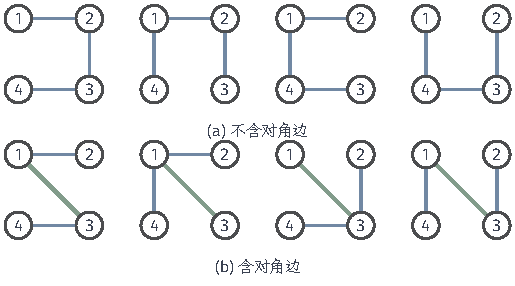
\includegraphics{figures/03-graphs/05-matrices-and-spectra/tikz/sparsification-spanning-trees/figure.pdf}
  \caption{四点五边单位权图的全部$8$棵生成树。上排$4$棵不含对角边$13$，下排$4$棵包含对角边$13$。每条环边（如$12$）在$8$棵树中出现$5$次，故$R_{1,2}=5/8$；对角边$13$在$8$棵树中出现$4$次，故$R_{1,3}=4/8=1/2$。}
  \label{fig:sparsification-spanning-trees}
\end{BookInlineFigure}

由于各边电导均为$1$，生成树包含概率$\mathbb P(e\in T)=c_e R_e$直接等于有效电阻$R_e$。观察图~\ref{fig:sparsification-spanning-trees}：以环边$12$为例，上排$4$棵树中有$3$棵包含它，下排$4$棵树中有$2$棵包含它，共计出现$5$次，故$R_{1,2}=\mathbb P(12\in T)=5/8$；对角边$13$恰好在下排$4$棵树中出现，故$R_{1,3}=\mathbb P(13\in T)=4/8=1/2$。这与第~\ref{sec:electrical-series-parallel}小节通过串并联和拉普拉斯方程算出的结果完全一致。

\subsubsection{Foster定理}
\label{sec:graph-foster-theorem}

对单条边而言，$c_e R_e\in(0,1]$给出了它在随机生成树中的出现概率；如果把全图所有边的$c_e R_e$加起来，总和是多少？由于每一棵生成树都恰好包含$n-1$条边，全图所有边的包含概率之和必定恒等于生成树的边数$n-1$——这就是电网络理论中著名的\term{Foster定理}（Foster's theorem）。

\begin{theorem}[Foster定理]
\label{thm:graph-foster-theorem}
对包含$n$个顶点的连通正权网络$\mathcal G=(V,E,c)$，全体边的电导与有效电阻乘积之和恒等于$n-1$：
\begin{equation}
\sum_{e\in E}c_eR_e=n-1.
\label{eq:graph-foster-sum}
\end{equation}
更一般地，若网络有$k$个正权连通分量，则$\sum_{e\in E}c_e R_e = n-k$。
\end{theorem}

\begin{proof}
我们给出两种相互印证的证明：一种利用随机生成树的期望，另一种利用拉普拉斯伪逆的矩阵迹。

方法一（生成树边数期望法）：在按式~\eqref{eq:graph-weighted-tree-distribution}抽取的随机生成树$T$中，对每条边$e\in E$定义零一指示随机变量$I_e(T)=\mathbb I(e\in T)$。由于任一棵生成树$T$恒有$n-1$条边，必有恒等式$\sum_{e\in E}I_e(T)=n-1$。对等式两边取数学期望，利用期望的线性性及定理~\ref{thm:graph-tree-edge-probability}的$\mathbb E[I_e(T)]=\mathbb P(e\in T)=c_e R_e$，立得
\[
\sum_{e\in E}c_eR_e = \sum_{e\in E}\mathbb P(e\in T) = \mathbb E\!\left[\sum_{e\in E}I_e(T)\right] = n-1.
\]

方法二（拉普拉斯伪逆求迹法）：将$R_e=\bm b_e^\top\bm L^\dagger\bm b_e=\operatorname{tr}(\bm L^\dagger\bm b_e\bm b_e^\top)$代入求和，利用迹的线性性及$\bm L=\sum_{e\in E}c_e\bm b_e\bm b_e^\top$，可得
\[
\sum_{e\in E}c_eR_e
=\operatorname{tr}\!\left(\bm L^\dagger\sum_{e\in E}c_e\bm b_e\bm b_e^\top\right)
=\operatorname{tr}(\bm L^\dagger\bm L).
\]
在连通图上，$\bm L^\dagger\bm L=\bm I-\frac{1}{n}\bm 1\bm 1^\top$是向$n-1$维零和子空间$\bm 1^\perp$上的正交投影矩阵，其迹等于子空间维数$\operatorname{dim}(\bm 1^\perp)=n-1$（当图有$k$个连通分量时，$\bm L$的零空间维数为$k$，投影矩阵的秩与迹均为$n-k$）。
\end{proof}

用四点五边单位权图核对Foster定理：$4$条环边的$c_e R_e$均为$5/8$，对角边的$c_e R_e$为$1/2$，五条边相加得$4\times\frac58+\frac12=3=n-1$。又如在单位权完全图$K_n$中，全部$\binom{n}{2}$条边地位完全对称，由Foster定理无需解方程即可直接读出任意两点间的有效电阻为$R_e=(n-1)/\binom{n}{2}=2/n$。在第~\ref{chap:graph-sparsification}章中，Foster定理给出的归一化常数$\sum_{e\in E}c_e R_e=n-1$将直接把$\{c_e R_e\}_{e\in E}$转化为边抽样概率分布$p_e=\frac{c_e R_e}{n-1}$。

\section{本章小结}
\label{sec:graph-electrical-networks-summary}

给定各顶点的外部注入后，逐边的电流守恒和Ohm定律联立为拉普拉斯方程$\bm L\bm v = \bm b$。正权连通分量内注入总量为零是有解的充要条件。接地选定电势基准——删去的那一列对应已固定的电势，删去的那一行可由其余方程恢复。非连通时各分量独立选基准，孤点注入必须为零。

同一组注入下，电流不唯一决定于守恒条件。不同的守恒流与实际电流之差是环流——它不改变任何顶点的净流出。叠加环流只增加该环流自身的耗散，交叉项因电势与环流正交而消去。实际电流因此是耗散最小的守恒分流，最小耗散同时等于两端压降。这把能量最小原理和有效电阻联系在一起。

计算方式取决于任务。查询单个点对时，解它的单位注入方程再取电势差。树上每条边的电流可以由一侧子树的注入和直接确定，电势由根向叶递推，时间为$O(n)$。若要查询大量点对，可以用一批随机右端给每个顶点预计算低维坐标，之后每次查询只需取两列的平方距离。投影维数和方程求解精度分别控制近似误差和失败概率。

有效电阻在稀疏化与行走中还会出现：第~\ref{chap:graph-sparsification}章用边的有效电阻决定抽样权重，第~\ref{chap:graph-walks}章用点对有效电阻计算随机游走的平均往返时间。

